\chapter{Evaluation} 
This chapter presents an evaluation of the initial results from the collected data focusing on statistics relating to
developmental trajectories in order to identify potential developmental indices. These findings serve as the
foundation
for the feature selection used in training the explainable boosting machine. Features that demonstrate strong
performance here may also be identified as important by the EBM. The following questions will be addressed in this
section:

\begin{enumerate}
    \item Which measures show an overall developmental trajectory across JLPT levels?
    \item Which features significantly discriminate between proficiency levels, and is a developmental trajectory
    apparent across these levels?
\end{enumerate}

\section{Complexity Measures}

Many of the complexity measures demonstrated trends that correspond to increasing proficiency. However, the patterns
varied across measures. Some showed a consistent increase,while others
decreased, or plateaued at the
higher levels. Notably, most measures were unable to distinguish between the N1 and native speaker (NS) groups.

Statistical analyses were conducted using ANOVA to test for significance, followed by Tukey's HSD test to identify
significant pairwise differences between adjacent proficency levels.

\subsection{Syntactic Complexity Measures}

%Sentence Length
    %discriminates between ajacent proficency levels.
%Clause per Sent
    %*Statistically significant difference between all adjacent levels except N1 and NS

Many of syntactic measures failed to show significant differences between N1 and NS groups. This however is not
cause for concern as the Native speaker group is not actually part of the JLPT scale and is used as a benchmark to
compare how close to native like speech the other learner's are. Therefore when it is mentioned that a measure
distinguished all adjacent levels this means all levels within the JLPT proficency scale not including the native
speaker group.
However several measures
such as sentence length, clauses per sentence, and coordinating clauses per sentence exhibited statistical significance
across most
adjacent proficency levels. These patterns are illustrated in Figures \ref{fig:sentLen}, \ref{fig:cpersent}, and
_____ respectively.

\begin{figure}[htbp]
    \centering
    \begin{minipage}{.48\textwidth}
        \centering
    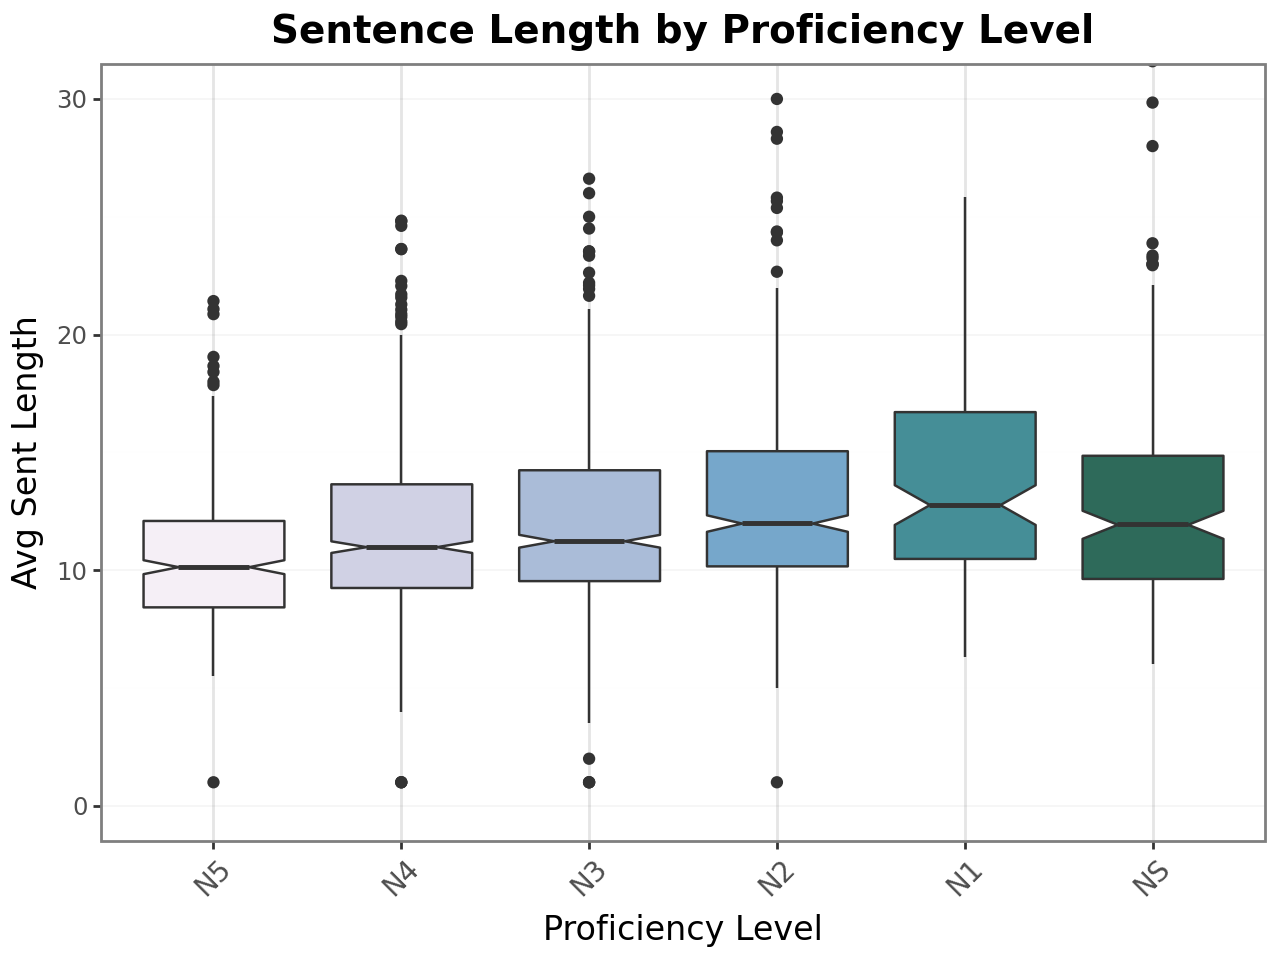
\includegraphics[scale=.3]{img/sentence_len}
    \caption[Average Sentence Length across JLPT levels]{Average Sentence Length across JLPT levels}
        \label{fig:sentLen}
    \end{minipage}
    \hfill
\begin{minipage}{.48\textwidth}
        \centering
        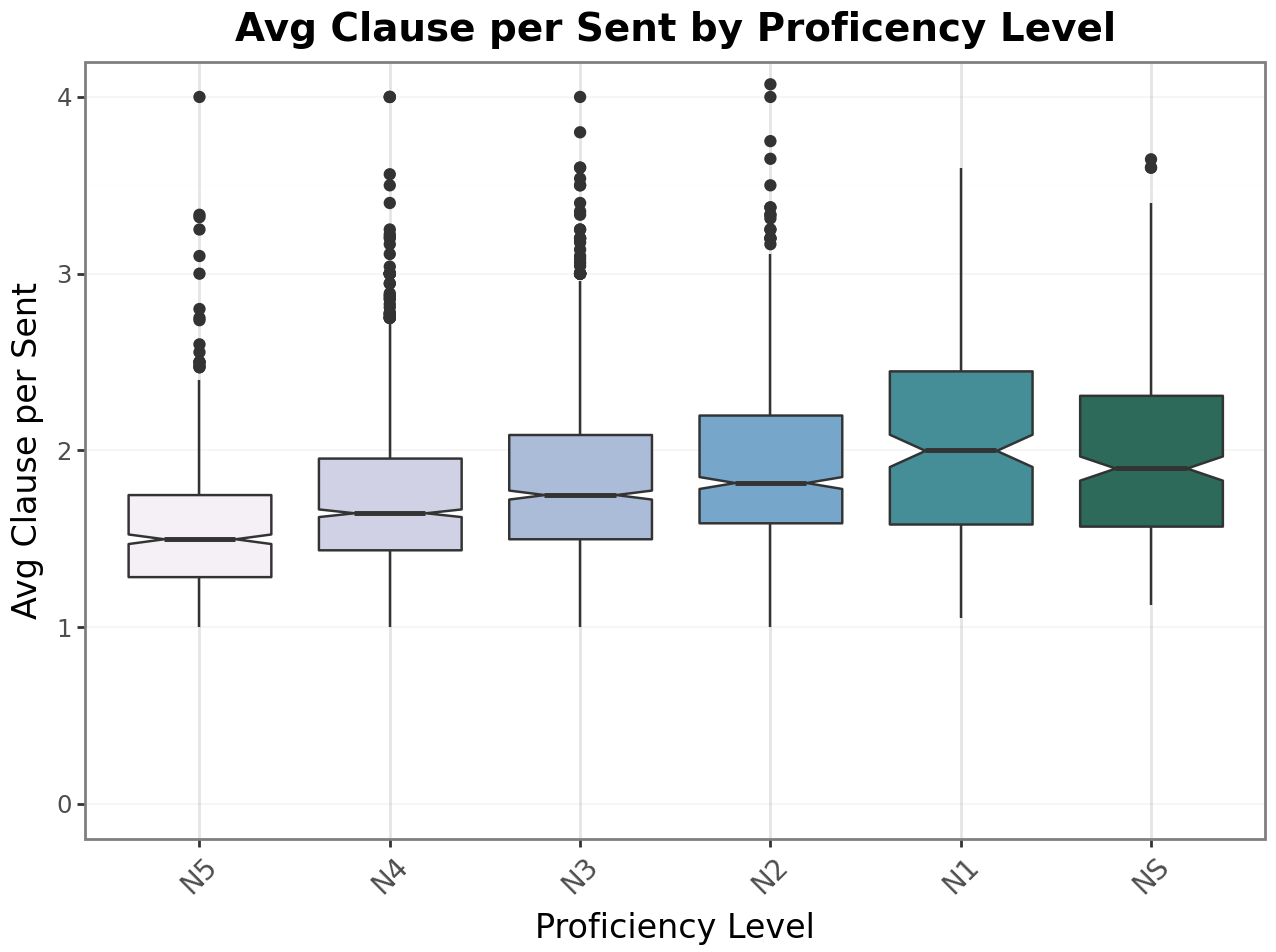
\includegraphics[scale=.3]{img/clausesSent}
        \caption[the ratio of clauses per sentence]{Plot showing the ratio of clauses per sentence}
\label{fig:cpersent}
\end{minipage}
    \end{figure}


\subsubsection{Length-Based Measures}

Length-based metrics capture the amount of syntactic material produced per unit (e.g. per sentence, per clause,
etc.) and are surface level-indications of syntactic complexity. Sentence length exhibited a general upward trend
across proficiency levels and was statistically significant at distinguishing across most adjacent levels, although
it failed to distinguish N1 from the NS group. This aligns
with
the idea that more advanced learners integrate more elements into a single sentence.

Noun phrase length and verb phrase length in contrast, were less informative. NP length remained relatively stable
and did not significantly differ across levels. Verb phrase length did show a weak upward trend but lacked
statistical significance to distinguish between the proficiency levels.

\subsubsection{Clause-Based Measures (Including Coordination/Subordination)}
Clause based measures focus on how learners structure and link clauses, capturing syntactic elaboration through
subordination and coordination.
%Clause Length
%    *N1 and N3 statistically significant difference observed
%    *slightly increases across levels.
%    *Could be influenced by tasks?. Try Removing SW1 and SW2 tasks

Clause length showed a slight
increase across proficiency levels, with a statistically significant difference in distinguishing between N1 and N3.
However, when the SW1 and SW2
tasks were removed, this measure distinguished between all adjacent upper proficiency levels, suggesting a at a
possible
task effect. increases in clause length were more pronounced at the advanced stages than at the beginner levels,
hinting at its potential in detecting finer gradiations of advanced proficiency.

%add other citations
Across prior studies on l2 syntactic development, a common finding is a decrease in coordination and an increase in
subordination with proficiency \citep{Vyatkina2012, Lu2010,Lu2011}. However, in the present data, this trend was not
entirely replicated. One reason may be the early introduction of subordinating conjunctions in Japanese L2
instruction such as 「から」(kara, \textit{because}) and 「けど」(kedo, \textit{but}) which are frequently used without
requiring transformation of verbs or deep syntactic embedding.

%Subordinate Clauses per Sent
    %statistically significance difference between N5 and N4 ,and then N1 and N3 but does not discriminate between the
%higher proficency
    %levels. Subordination is taught quite early to L2 speakers, could this be why?
%Subordinate Clause per clause
    %statistically significant difference between N5 and N4 and N4 and N3,
    %slight decrease across levels showing a prefernce for different clause types in the higher levels?

The measure of subordinate clauses per sentence showed a modest increase across proficiency levels and was
statistically significant in distinguishing lower levels(N5 vs N4) and non-adjacent upper levels (N3 vs N1). This
reflects developmental progression but not ina  linear fashion (see Figure~\ref{fig:SubclperS}).

In contrast, the ratio of subordinate clauses to total clauses showed a decreasing trend, with significant
differences observed between non-adjacent levels (N5 vs N3, N4 vs N2).  As shown in Figure~\ref{fig:SCperC}, this
suggests that lerners at higher proficiency levels may diversify their clause structures and shift toward more
coordination or other complex constructions.

\begin{figure}[htbp]
    \centering
    \begin{minipage}{.48\textwidth}
        \centering
    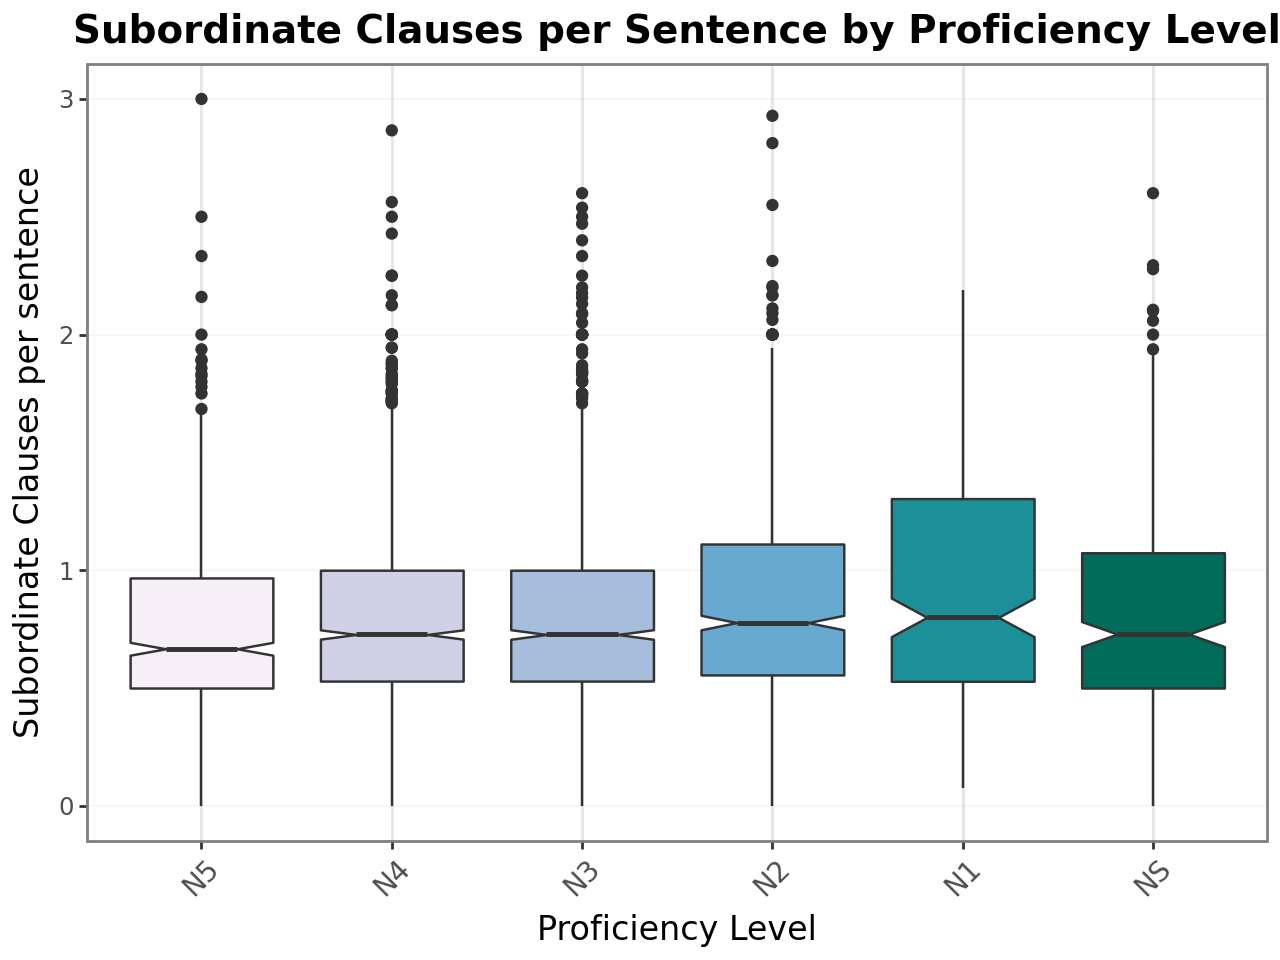
\includegraphics[scale=.3]{img/SCperS}
    \caption[Average subordinate clauses to sentences across JLPT levels]{Average subordinate clauses to sentences across JLPT levels}
        \label{fig:SubclperS}
    \end{minipage}
    \hfill
\begin{minipage}{.48\textwidth}
        \centering
        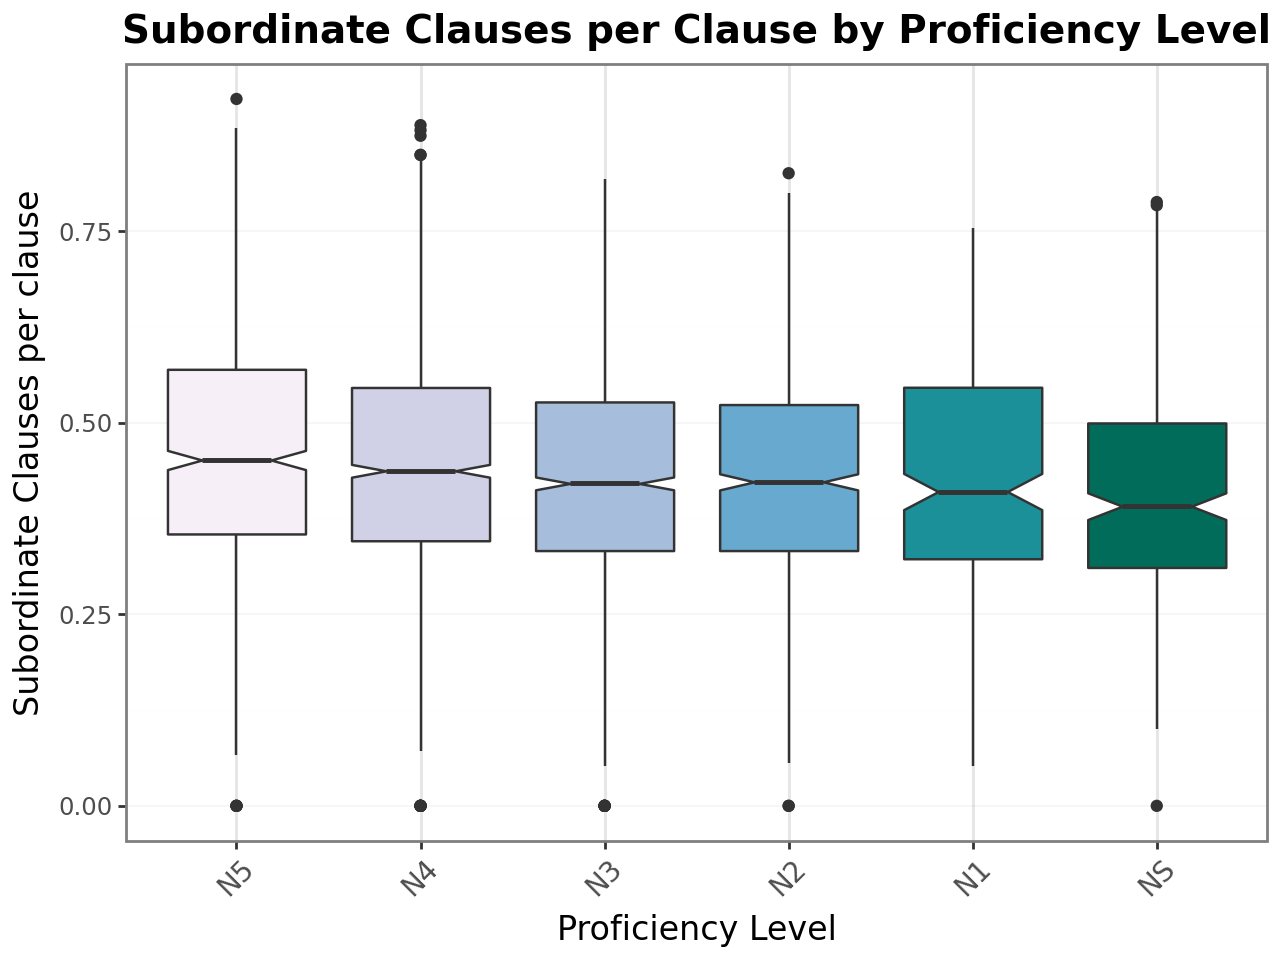
\includegraphics[scale=.3]{img/SCperC}
        \caption[Average subordinate clauses to clauses ratio across JLPT levels]{Average subordinate clauses to clauses ratio across JLPT levels}
\label{fig:SCperC}
\end{minipage}
    \end{figure}

%Coordinating Conjunction per Sentence
    %*Statistically significant in distinguishing all adjacent levels except N1 and NS group
    %*Also increases across prof levels, could be due to the fact that SC are taught first.
%Coordinating Conjunction per Clause
    %*increase across prof. levels
    %*Statistically significant between levels except N2 & N1 and N1 & NS
%Subordinating Clauses to Coordinate Clauses
%    *statistically significant for every other proficency level. ie. N5 & N3, N3 & N1, N2&N4
%    *variance also increases at the higher proficency levels but , maybe due to more CC being used?

Measures related to coordination showed strong developmental patterns. The number of coordinate clauses per sentence
increased across levels and significantly
distinguished all adjacent levels. This trend may reflect increased syntactic range at higher levels where
coordination is used stylistically or rhetorically, not just structurally (Figure~\ref{fig:CCperSent}).

Similarly, coordinate clauses per clause also increased with proficiency and distinguished most adjacent levels
except N2 - N1 (Figure~\ref{fig:CCperCl}). These findings contrast with typical L2 development models by maybe due
to the instructional sequence in Japanese, where simple subordinate forms are taught earlier and coordination
becomes more common as learners diversify their expression.

The ratio of subordinate clauses to
coordinate clauses further supports this shift. It showed statistically significant differnces between non-adjacent
levels (N5 vs N3, N3 vs N1) and increased variance at higher proficiency levels, possibly reflecting more
individualized or task-drive distribution of clause types.

\begin{figure}[htbp]
    \centering
    \begin{minipage}{.48\textwidth}
        \centering
    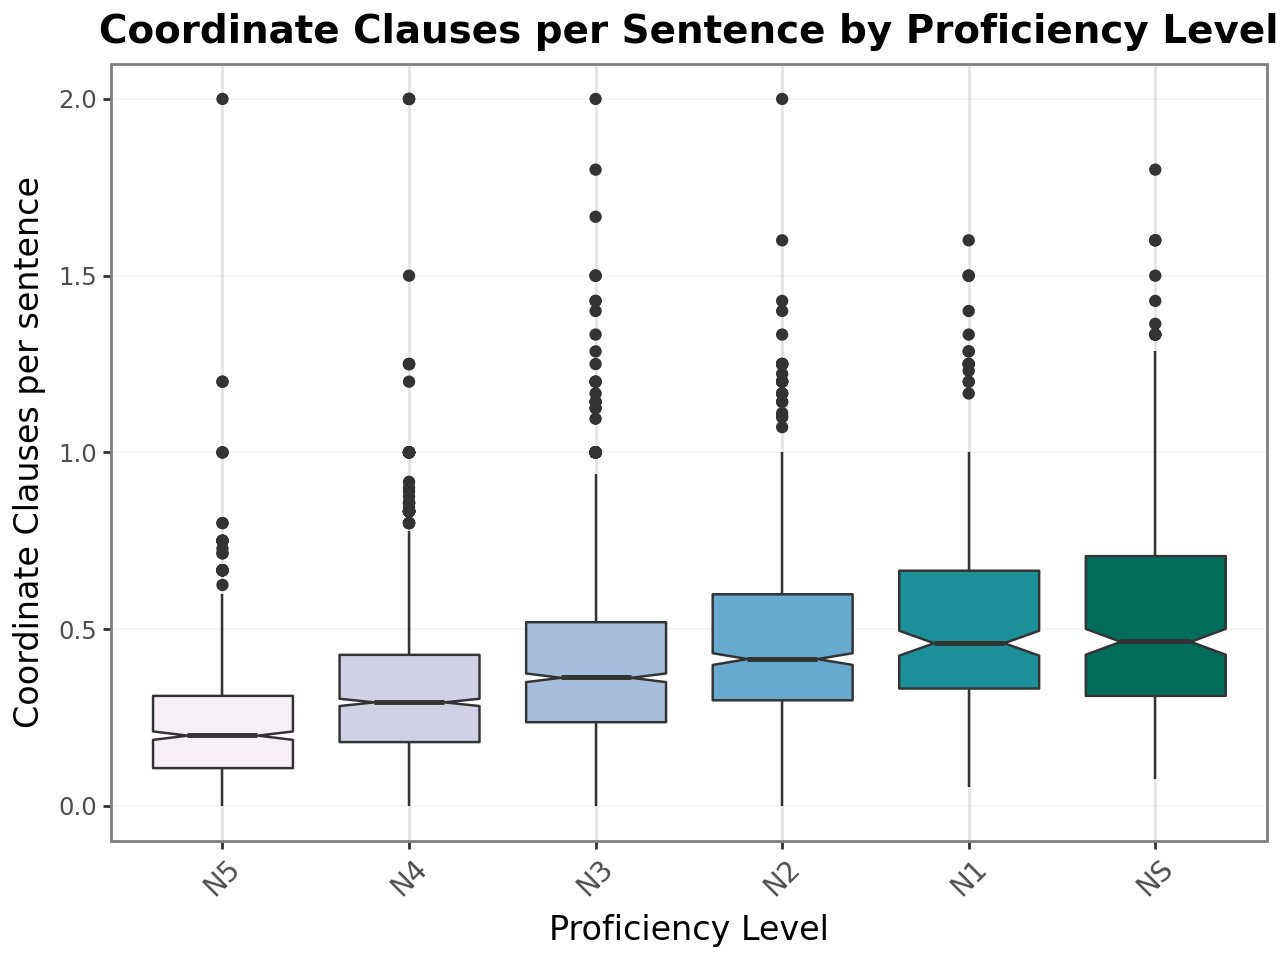
\includegraphics[scale=.3]{img/CCperSent}
    \caption[Average coordinate clauses to sentences across JLPT levels]{Average coordinate clauses to sentences across JLPT levels}
        \label{fig:CCperSent}
    \end{minipage}
    \hfill
\begin{minipage}{.48\textwidth}
        \centering
        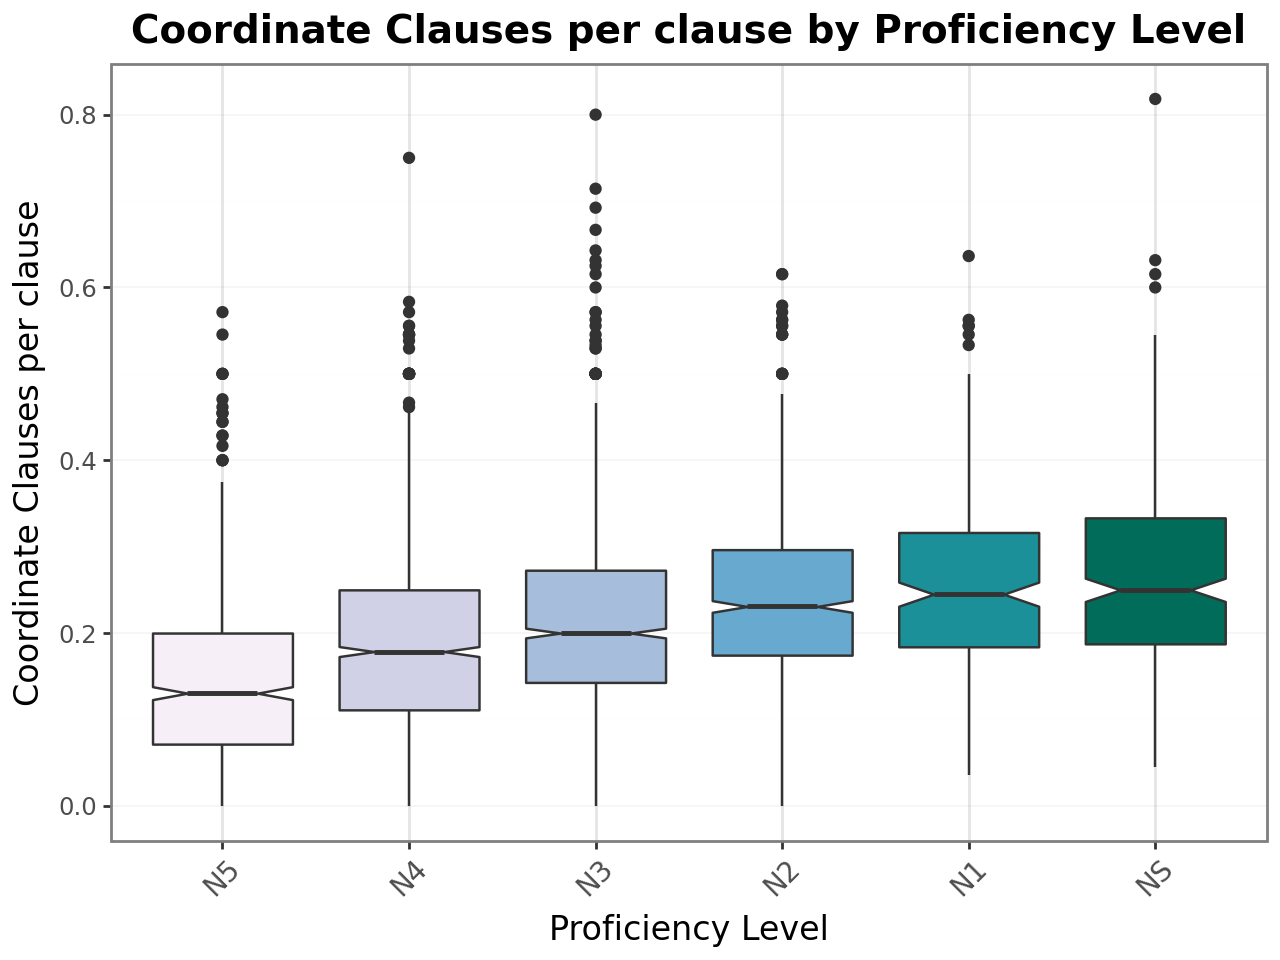
\includegraphics[scale=.3]{img/CCperC}
        \caption[Average coordinate clauses to clauses ratio across JLPT levels]{Average coordinate clauses to clauses ratio across JLPT levels}
\label{fig:CCperCl}
\end{minipage}
    \end{figure}

%CC Freq
    %no significant difference between any of the levels and no clear pattern...
%SC Frequency
    %*increases across levels
    %*Significant between n5&N4, N4&N3, N3&N2, N2 & NS
Normalized frequencies of subordinating and coordinating conjuctions were analyzed as a proxy measure as done in \citet{Vyatkina2012}, however, they showed mixed results. Subordinating conjunction frequecy increased across proficiency levels and showed statistically significant differences at lower levels (N5 vs. N4, N4 vs N3), reflecting early acquisition and frequent use. Coordinating conjunction frequency, however, did not show significant variation across levels and did not follow a clear developmental trend. This may be due to extraction limitations or the realtively sparse distribution of explicit coordinators in learner texts.

\subsubsection{Dependency-Based Measures}

Dependency-based measures provide a structural perspective on syntactic complexity by quantifying how syntactic
units are hierarchically and linearly related. Unlike length or clause-based measures, which capture surface level
elaboration, these metrics reflect the cognitive load and integration required to process or produce a sentence.
Both measures considered, Mean Dependency Distance (MDD) and Mean Hierarchical Distance (MHD), showed strong
associations with increasing proficiency and can be considered promising indicators of developmental progression.

%MDD
    %* Statistically significant between every other level as well as the higher proficency levels N3&N2 and N2&N1
    %*no significant between N1 and NS
    %*Increase across levels
As shown in Figure~\ref{fig:mdd}, MDD increased consistently across proficiency levels and was statistically
significant between most levels, including higher-level distinctions such as N3 vs. N2 and N2 vs. N1. The consistent
upward trajectory suggests that as learners become more proficient, they are able to manage longer dependency
relations, producing more integrated syntactic structures.

%MHD
%    *Increase across levels
%    *statistically significant between all adjacent levels except NS and N1

Similarly, MHD, depicted in Figure~\ref{fig:mhd}, also exhibited a steady increase with proficiency. It was
statistically significant across all adjacent levels. This measure captures the hierarchical depth of sentence
structure, and its strong performance across levels supports the idea that syntactic embedding becomes more complex
and frequent as learners advance.

\begin{figure}[htbp]
    \centering
    \begin{minipage}{.48\textwidth}
        \centering
    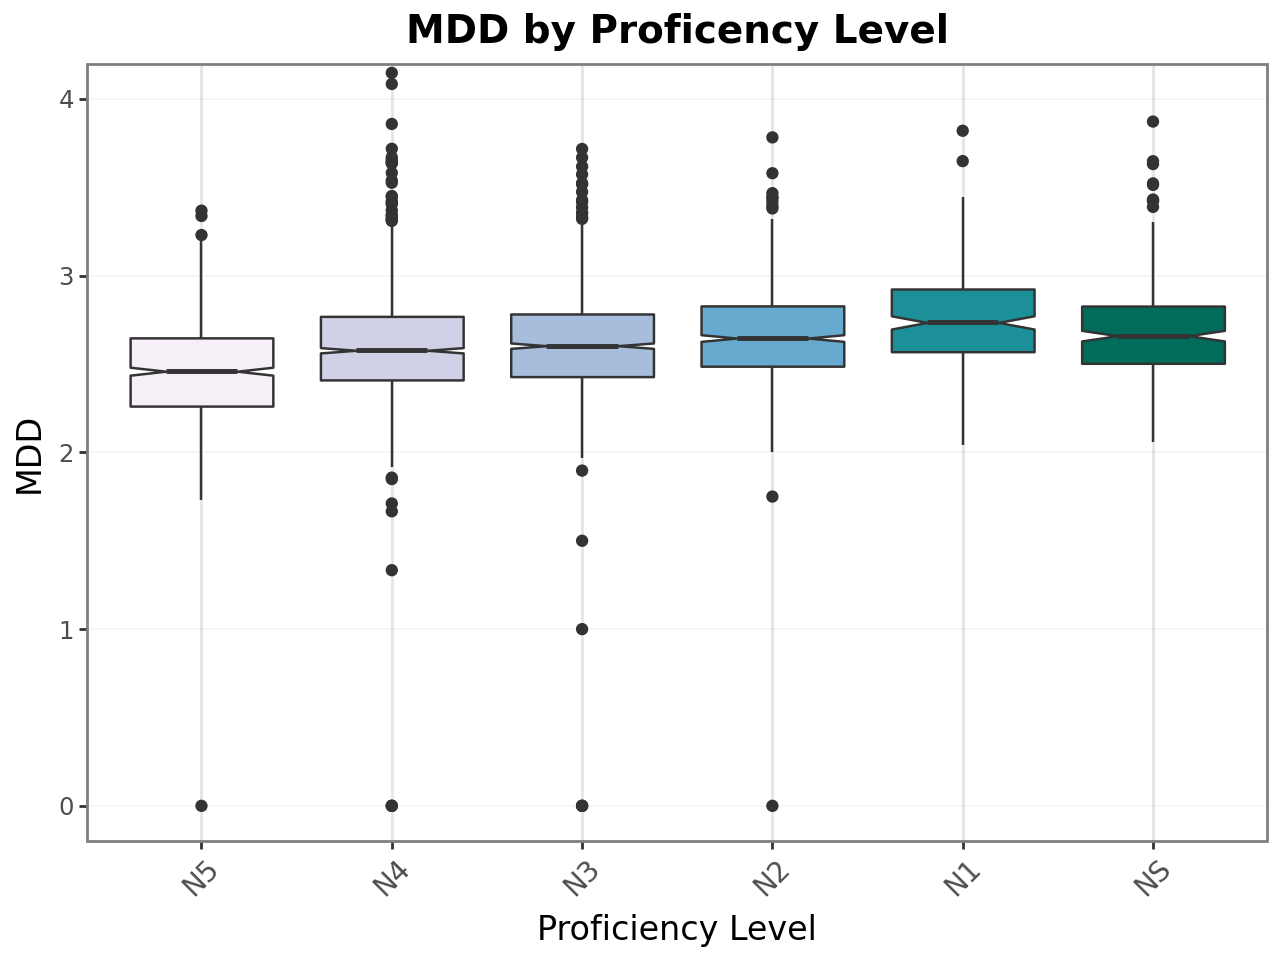
\includegraphics[scale=.4]{img/MDD}
    \caption[Mean Dependency Distance across JLPT Proficency Levels]{Mean Dependency Distance (MDD) increases steadily across JLPT levels, with significant differences between most levels.}
        \label{fig:mdd}
    \end{minipage}
    \hfill
\begin{minipage}{.48\textwidth}
        \centering
        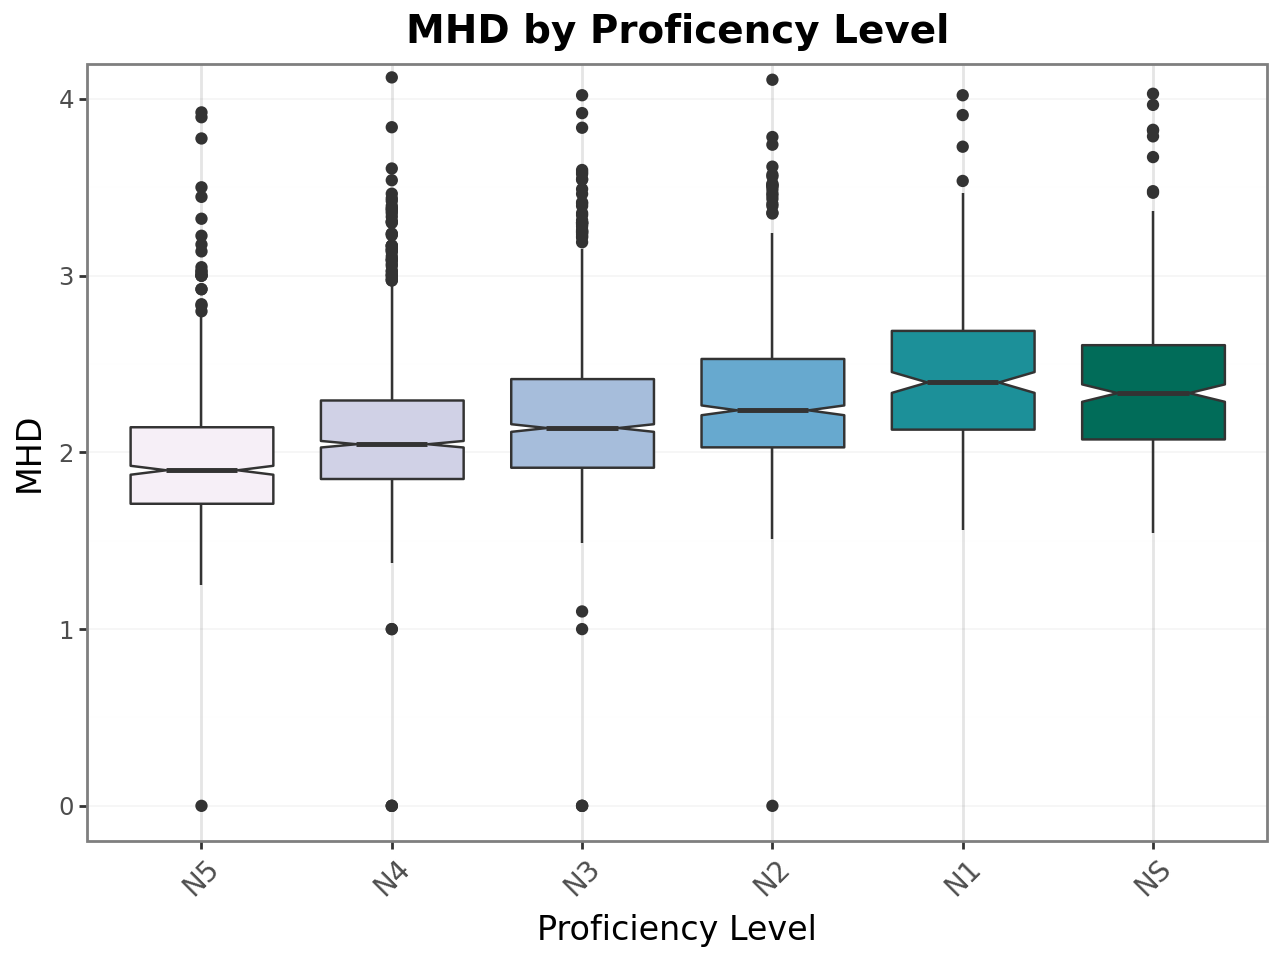
\includegraphics[scale=.4]{img/MHD}
        \caption[Mean Hierarchtical Distance across JLPT Proficency Levels]{Mean Hierarchtical Distance (MHD) increases consistently, distinguishing all adjacent proficency levels.}
\label{fig:mhd}
\end{minipage}
    \end{figure}


\subsection{Lexical Complexity Measures}
Lexical complexity captures the diversity, sophistication and density of vocabulary used by learners. The measures
included to evaluate how vocabulary use changes across proficiency levels include type-based diversity metrics, part
-of-speech (POS) density ratios, and lexical frequency profiles.

\subsubsection{Lexical Diversity Measures}
%CTTR
%    *Discriminates between adjacent levels at the lower proficiency levels,but no statistical significant difference
%    found between N2 & N1 and N1 & NS, and N2 and NS
%    *Generally increases between levels

The Corrected Type-Token Ratio (CTTR) showed a general increase across proficiency levels but was most effective at
distinguishing between adjacent levels in the lower proficiency range (Figure~\ref{fig:cttr}). No statistically significant
differences were
found between N2 vs. N1. This suggests that CTTR may plateau at advanced levels and is more sensitive to early
vocabulary expansion.

\begin{figure}[h]
    \centering
    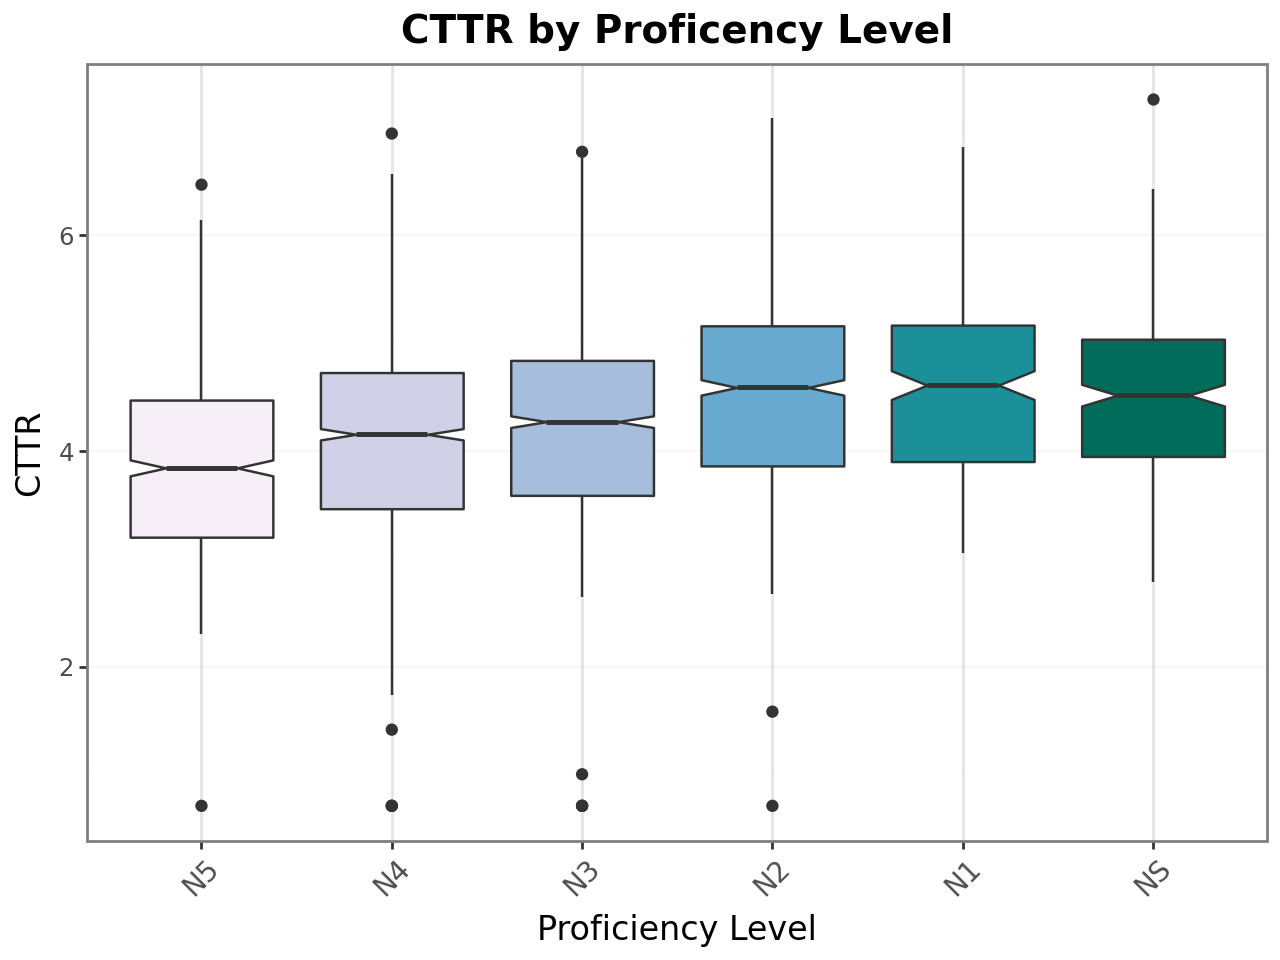
\includegraphics[scale=.5]{img/CTTR}
    \caption[Correct-Type]{CTTR}
    \label{fig:cttr}
\end{figure}

%MTLD-Surface
    %* increases across levels
    %* Statistically significant in distinguishing between lower prof levels.('N2', 'N3'), ('N2', 'N4'), ('N3', 'N5')
%, ('N4','N5')
%MTLD-Inflection
    %*increases across levels not as much as with surface forms
    %* Statistically significant in distinguishing between lower prof levels.('N2', 'N3'), ('N2', 'N4'), ('N3', 'N5')
%, ('N4','N5')

The Measure of Textual Lexical Diversity was calculated for surface forms and lemmas (non-inflected forms). The
MTLD-surface measure increased steadily across proficiency levels and showed statistically significant differences
for several adjacent pairs in the lower and mid-proficiency ranges (N5 vs. N4, N3 vs. N2). This suggest a gradual
increase in word variety as learners develop their langauge (Figure~\ref{fig:mtldS}). The MTLD-lemma measure also
showed an increasing trend, although the effect size was smaller than for surface forms(Figure~\ref{fig:mtldL}). Statistically
significant
differences were observed between similar level pairs, suggesting that while learners increase their morphological
variation, this dimension of diversity develops more slowly.


\begin{figure}[htbp]
    \centering
    \begin{minipage}{.48\textwidth}
        \centering
    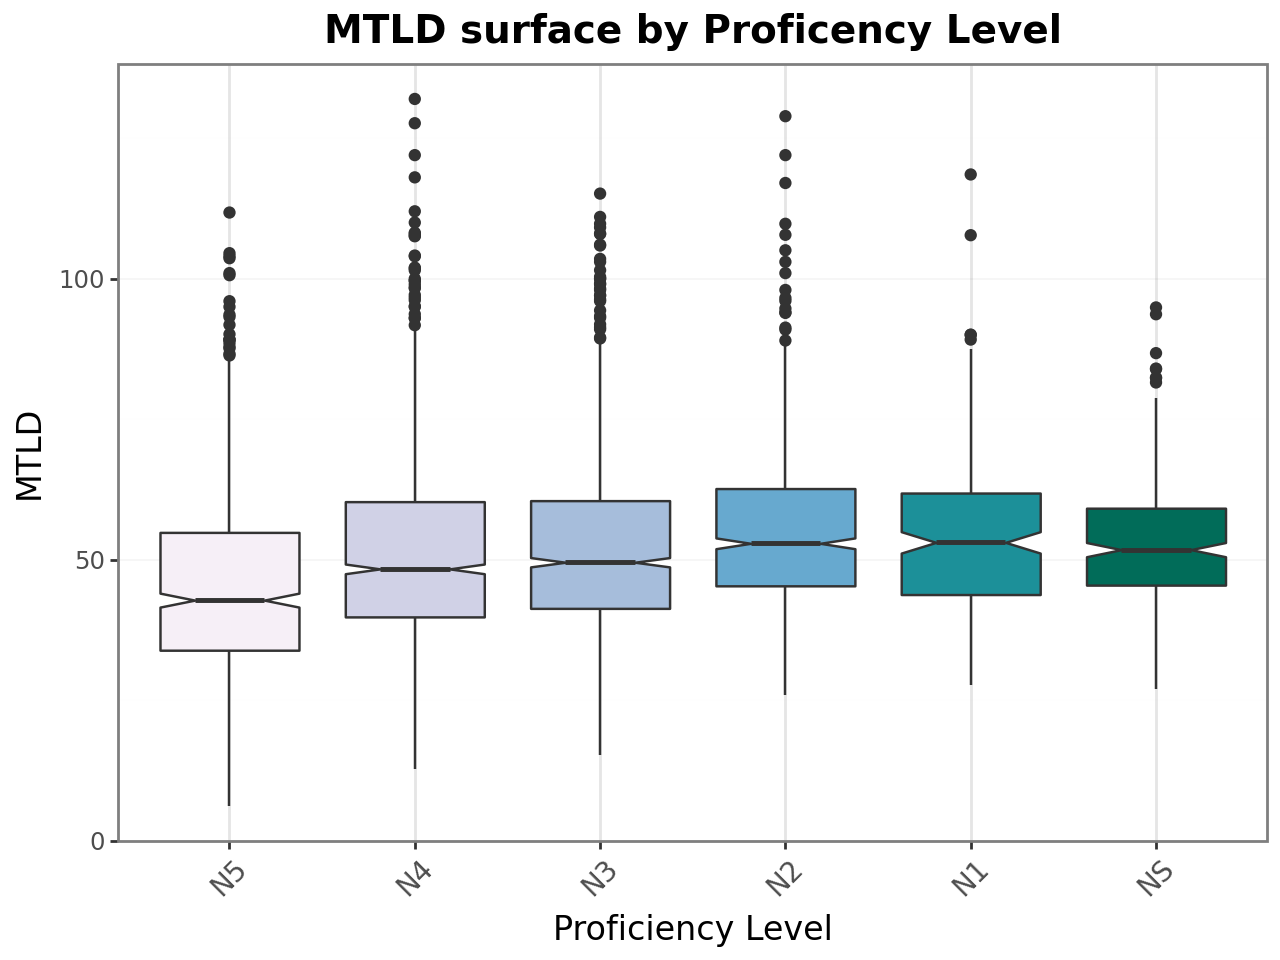
\includegraphics[scale=.4]{img/MTLDsurface}
    \caption[MTLD Surface]{MTLD Surface}
        \label{fig:mtldS}
    \end{minipage}
    \hfill
\begin{minipage}{.48\textwidth}
        \centering
        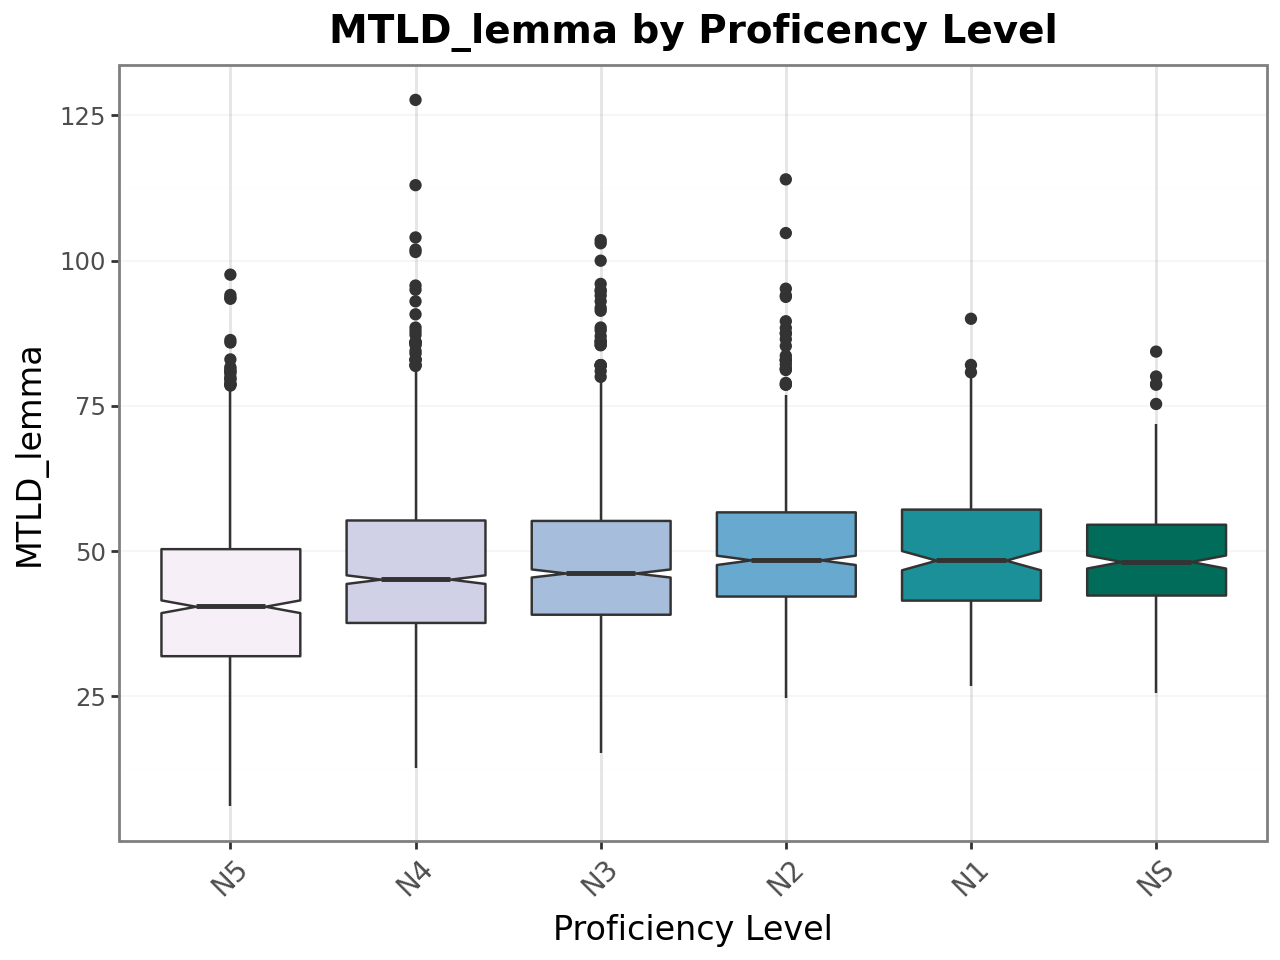
\includegraphics[scale=.4]{img/MTLDlemma}
        \caption[MTLD lemma]{MTLD Lemma}
\label{fig:mtldL}
\end{minipage}
    \end{figure}

\subsubsection{Lexical Density Measures}

Part-of-speech density ratios provide insight into how learners balance content and function words in their writing.
These ratios were normalized by total token count
%Noun Density
    %*Decreases across proficiency levels (null subjects?)
    %*distinguishes beteween lower prof levels. N4 & N5 and N3 and N4 (almost significant p = .06)
%Verb Density
    %*increase across levels
    %* Only statistically significant at distinguishing between lower levels N5 & N4 and N4&N3
Noun density decreased across proficiency levels. This may partially be explained by the use of null subjects in
Japanese, leading to fewer overt noun phrases in more advanced writing (Figure~\ref{fig:nounDen}). Statistically significant
differences were
observed between N5-N4 and N4-N3.

Verb density increased with proficiency but plateaued at the more advanced levels (Figure~\ref{fig:verbDen}) and was only
statistically
significant in distinguishing between the lower adjacent levels (N5-N4 and N4-N3). This pattern suggents that while
verb use expands early, it stabilizes in the upper ranges.

\begin{figure}[htbp]
    \centering
    \begin{minipage}{.48\textwidth}
        \centering
    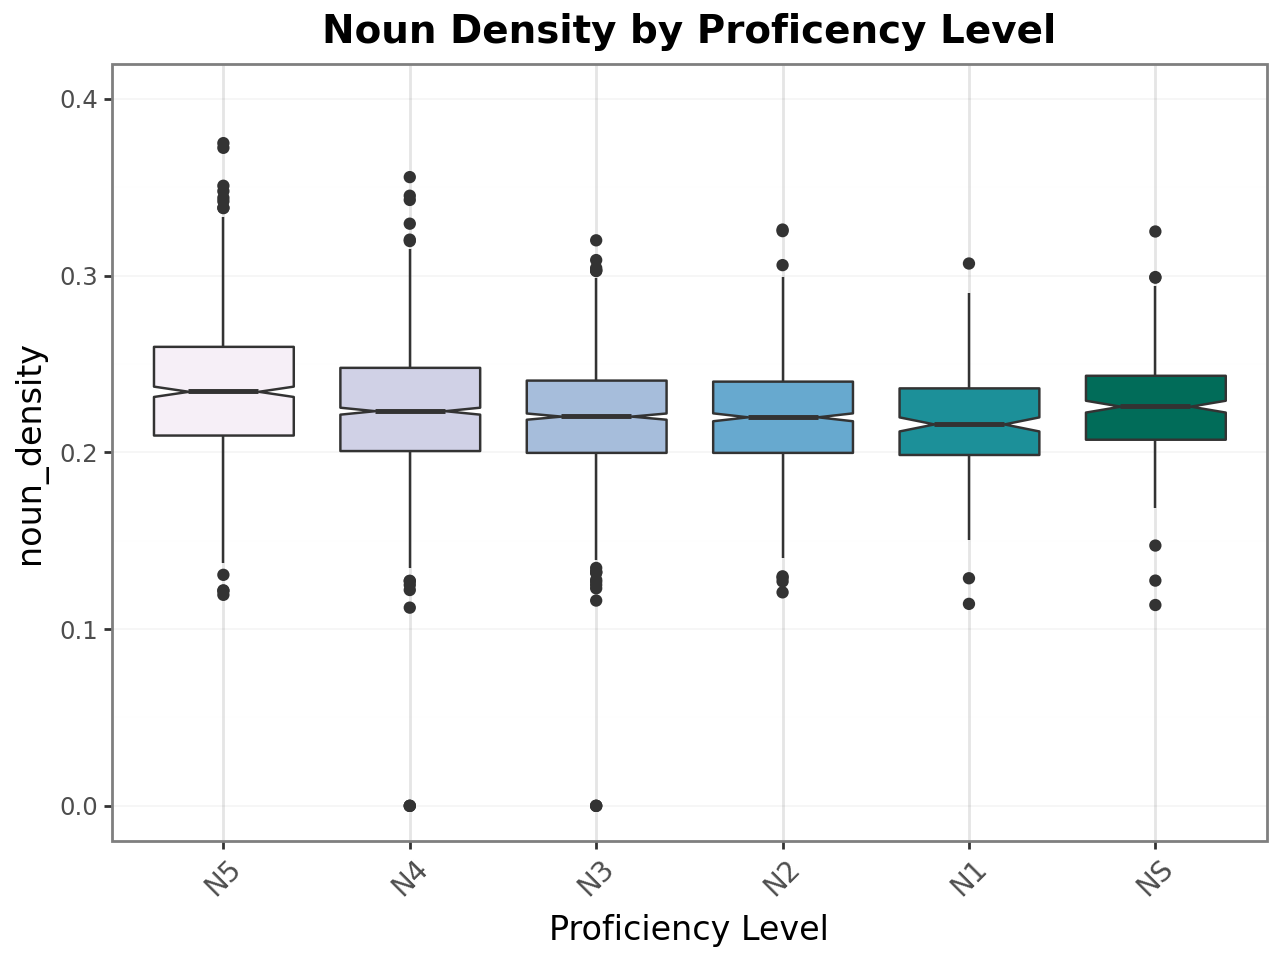
\includegraphics[scale=.4]{img/NounDen}
    \caption[Noun Density Across JLPT Proficiency Levels]{Noun Density}
        \label{fig:nounDen}
    \end{minipage}
    \hfill
\begin{minipage}{.48\textwidth}
        \centering
        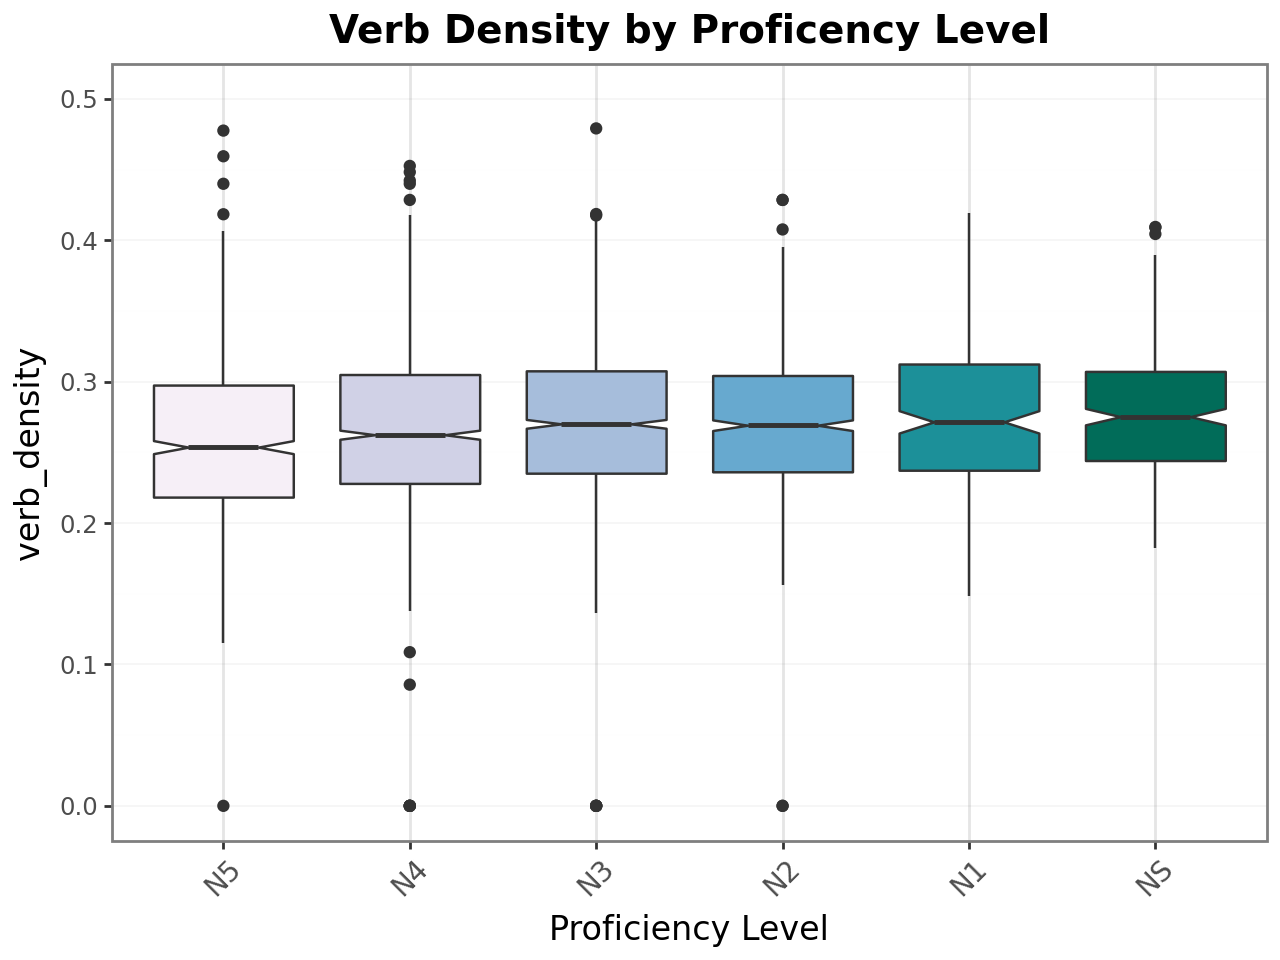
\includegraphics[scale=.4]{img/VerbDen}
        \caption[Verb Density Across JLPT Proficiency Levels]{Verb Density}
\label{fig:verbDen}
\end{minipage}
    \end{figure}


%Adjective Density
    %*Increase across proficiency levels
    %*Statistically significant in distinguishing between lower levels N5&N4, N5&N3, N3&N2
    %*could also be task dependent check later
%Adverb Density
    %*increase across levels except a drop in use for N1 (due to low sample size?)
    %*Statistically significant in distinguishing between lower levels N4&N5, N3&N5 N3&N2
Adjective density showed a consistent increase across proficiency levels and was statistically significant in
distinguishing lower and intermediate pairs (N5-N4, N5-N3, N3-N2). Adverb density also increased across levels, though with a noticeable drop at N1. This may be due to sample size
limitations or task variation. Statistically significant differences were found between N5-N4, N5-N3, and N3-N2,
indicating usefulness in assessment of early-stage proficiency.

\begin{figure}[htbp]
    \centering
    \begin{minipage}{.48\textwidth}
        \centering
    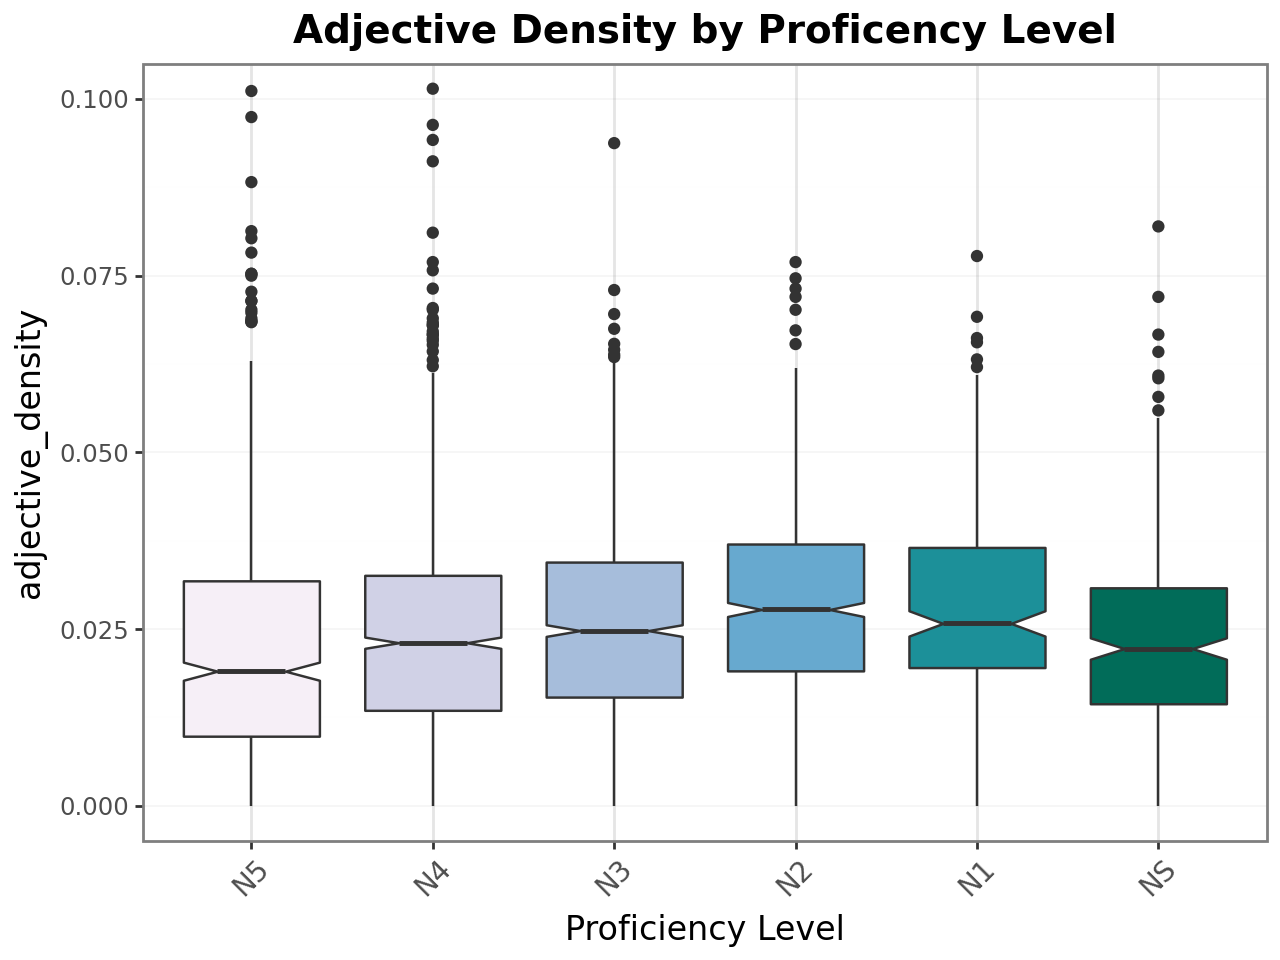
\includegraphics[scale=.4]{img/AdjDen}
    \caption[Adjective Density Across JLPT Proficiency Levels]{Adjective Density}
        \label{fig:adjDen}
    \end{minipage}
    \hfill
\begin{minipage}{.48\textwidth}
        \centering
        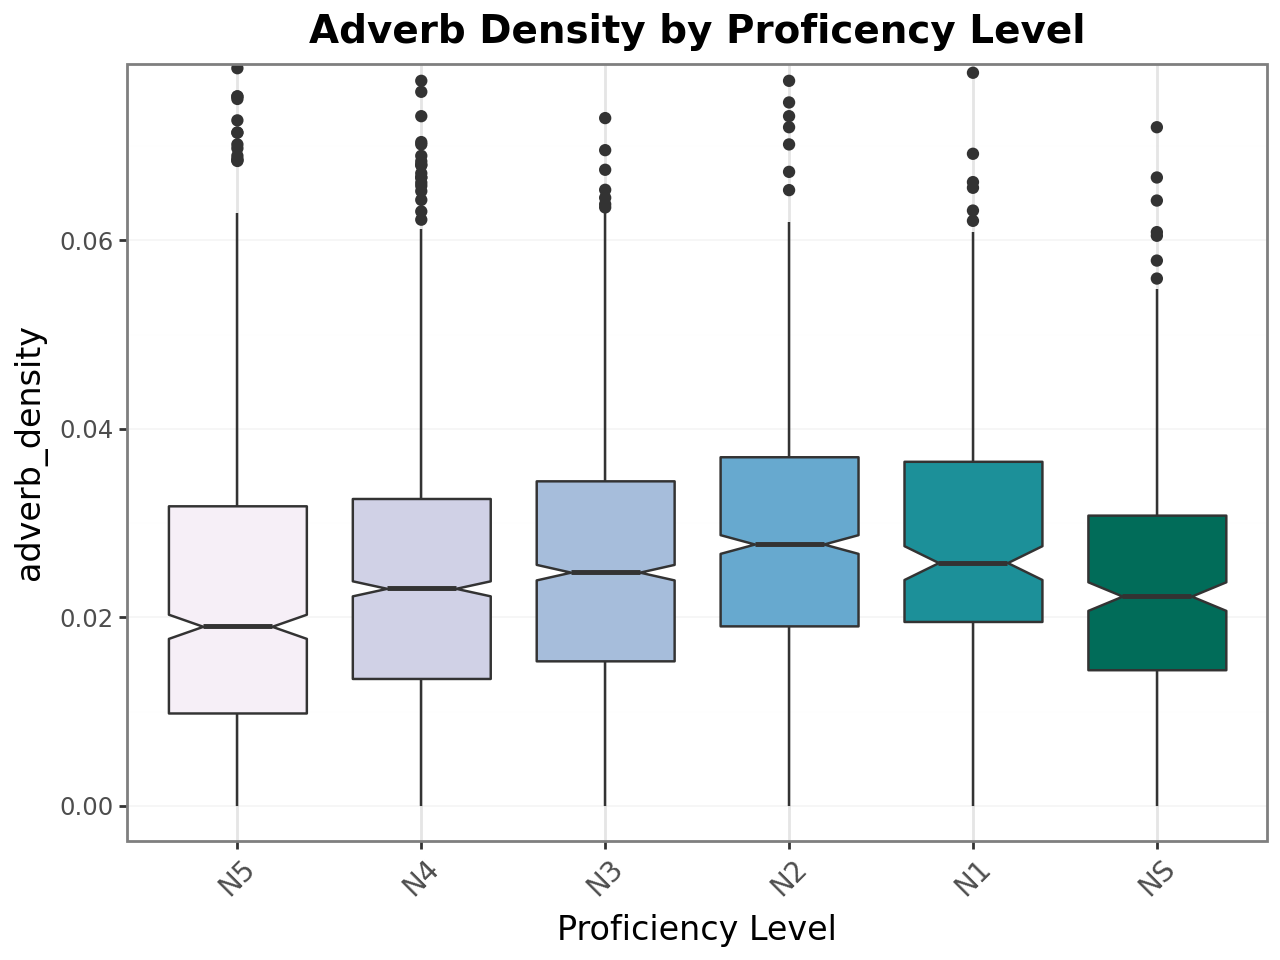
\includegraphics[scale=.4]{img/AdvDen}
        \caption[Adverb Density Across JLPT Proficiency Levels]{Adverb Density}
\label{fig:advDen}
\end{minipage}
    \end{figure}

\subsubsection{Lexical Frequency Profile Measures}
Lexical sophistication was examined using the Lexical Frequency Profile (LFP), and calculated based on two
reference corpora: the
Balanced Corpus of
Contemporary Written Japanese (BCCWJ) \citep{maekawa2014} and a JLPT-aligned wordlist \citep{jisho.org}. This
analysis aimed to capture how learners distribute their vocabulary use across frequency bands (in case of BCCWJ) or
across JLPT levels,
as their proficiency develops.

%LFP -BWCCJ Corpus
    %* high frequency of items in top 1,000 band across all proficiency levels
    %*N1 and Ns group had the largest raw count of vocab used across each band
    %* MANOVA revealed P value of Exact Wilks' Lambda p-value for JLPT 4.4492403847988e-133 meaning statistically
    %significant difference exists between bands, Taking a closer look at the individual bands....
        %*1k Band ->N5&N4, N2&N3, N1&NS, Percentage of vocab from 1k band decreases as
%proficiency increases.
        %especially at teh higher proficiency level.
        %*2K Band in contrast to 1k band the 2k band sees increase in percent of vocab used across proficiency levels ,
%same for the following bands as well, even if the actual frequency decreases as explained by zipfs distribution.
%No significant difference between N1 & NS group even though there is across the other bands.
%* because of low frequency in the higher bands statistical significance between levels is From 6k band onward no
%significant statistical difference observed between any of the levels, most likely due to low frequency. because of
%this bands 6 and onwards were removed from plots, etc.

%*Out of Vocabulary - decreases across proficiency levels, perhaps due to more errors in beginnger texts? statistical
%significant between N1 and NS group as well as the beginner levels, N5&N4 and N4&N3


In the BCCWJ-based analysis, words were grouped into 1,000 word frequency bands ranging for the most frequent (1k)
to the
least frequent (10k), with an additional category for out-of-vocabulary (OOV) words. As expected, across all JLPT
levels, most lexical tokens came from the 1k band(Figure~
\ref{fig:percentBands}). A multivariate analysis of variance (
MANOVA)
confirmed that significant differences existed between JLPT levels (p<.001). Closer examination revealed that the
portion of vocabulary from the 1k band decrease in usage as proficiency increased, especially at higher levels(Figure~
\ref{fig:1kband}). Significant pairwise differences were observed between N5-N4, N3-N2, and N1-NS, suggesting that
reliance of high frequency vocabulary diminishes with proficiency.


\begin{figure}[htbp]
    \centering
    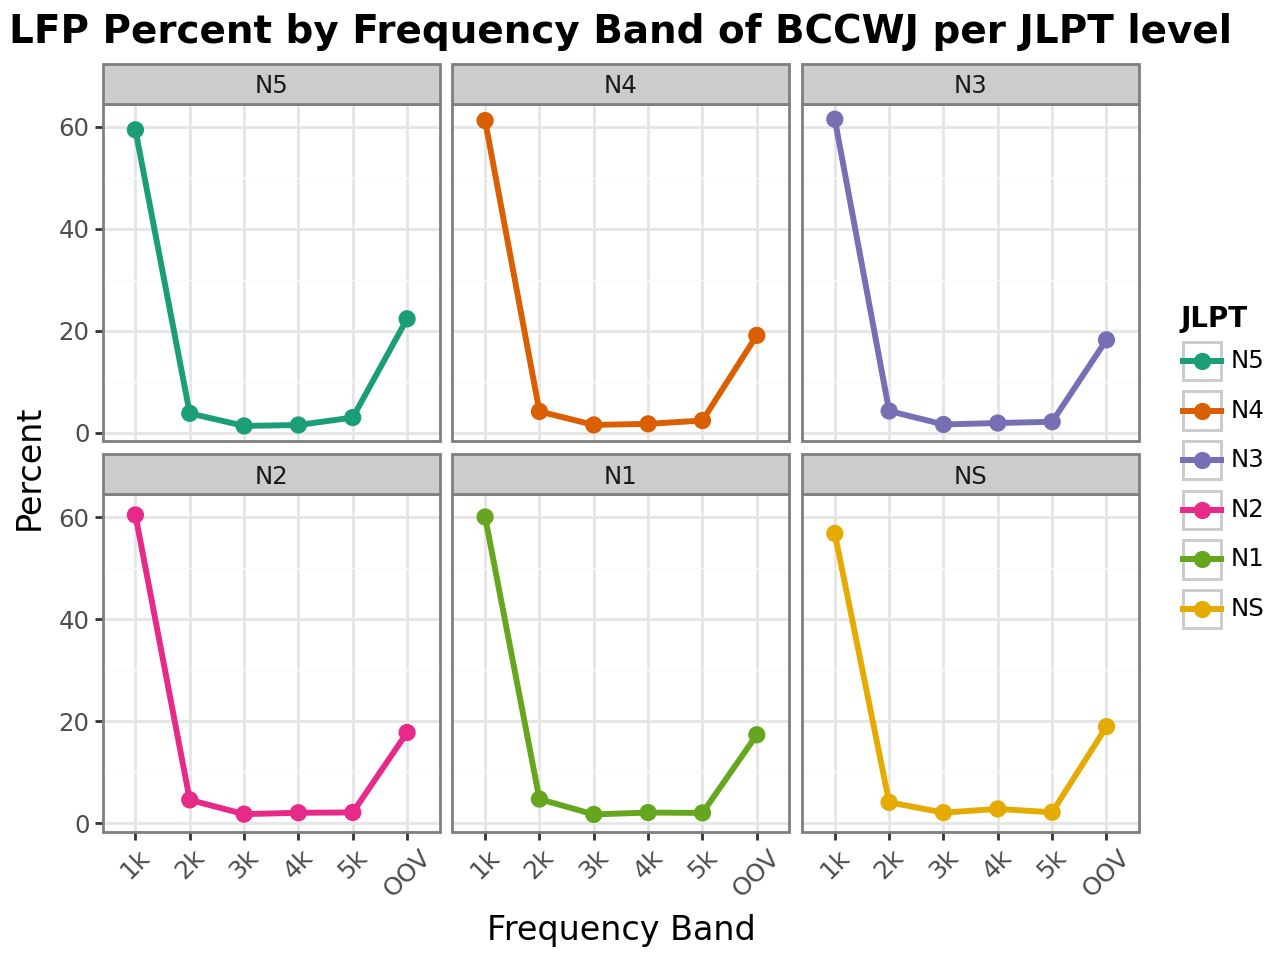
\includegraphics[scale=.4]{img/LFP/percentBands}
    \caption[A chart of the distribution of the average percent of tokens used across frequency band]{A chart of the precentage of tokens used across frequency bands}
    \label{fig:percentBands}
\end{figure}

In contrast, vocabulary from the 2k to 4k bands showed an updated trend in usage across proficiency levels,
indicating a broadening lexical range among more advanced learners. Despite these increases, the total token count
in these bands remains relatively low due to the natural distribution of word frequencies (Zipf's Law).
Nevertheless, the 2k band showed significant differences between non-adjacent levels (e.g. N5-N3 and N4-N2), and
similar patterns were observed for the 3k and 4k bands.

From the 5k band onward, useage declined steeply, and no statistically
significant differences were observed between proficiency groups. Given their low useage and minimal disriminatory
power, bands
5k through 10k were excluded from further analysis and visualization.


\begin{figure}[htbp]
    \centering
    \begin{minipage}{.48\textwidth}
        \centering
    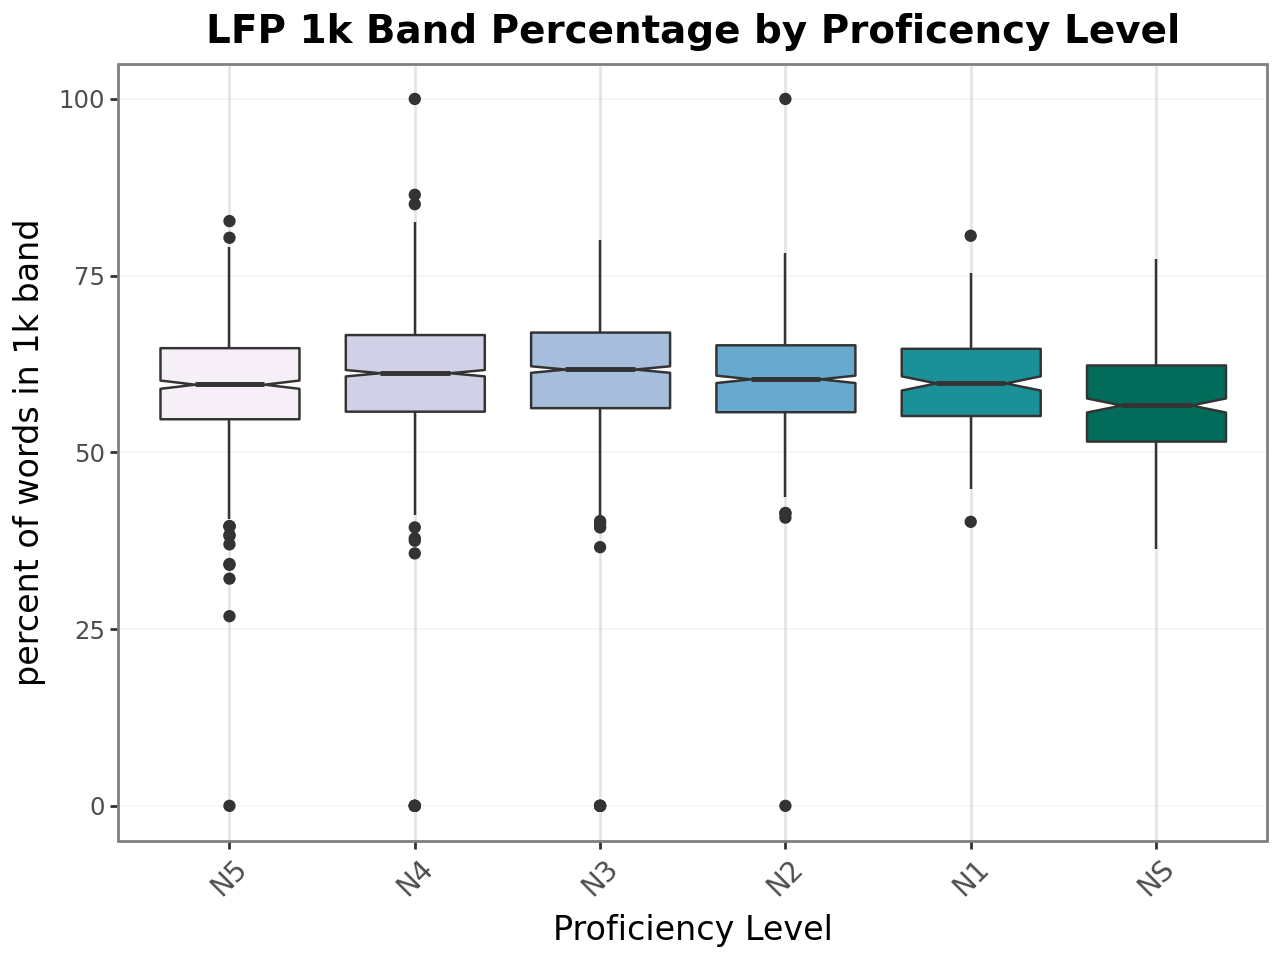
\includegraphics[scale=.4]{img/LFP/1k}
    \caption[Percentage of tokens used from 1k band]{}
        \label{fig:1kband}
    \end{minipage}
    \hfill
\begin{minipage}{.48\textwidth}
        \centering
        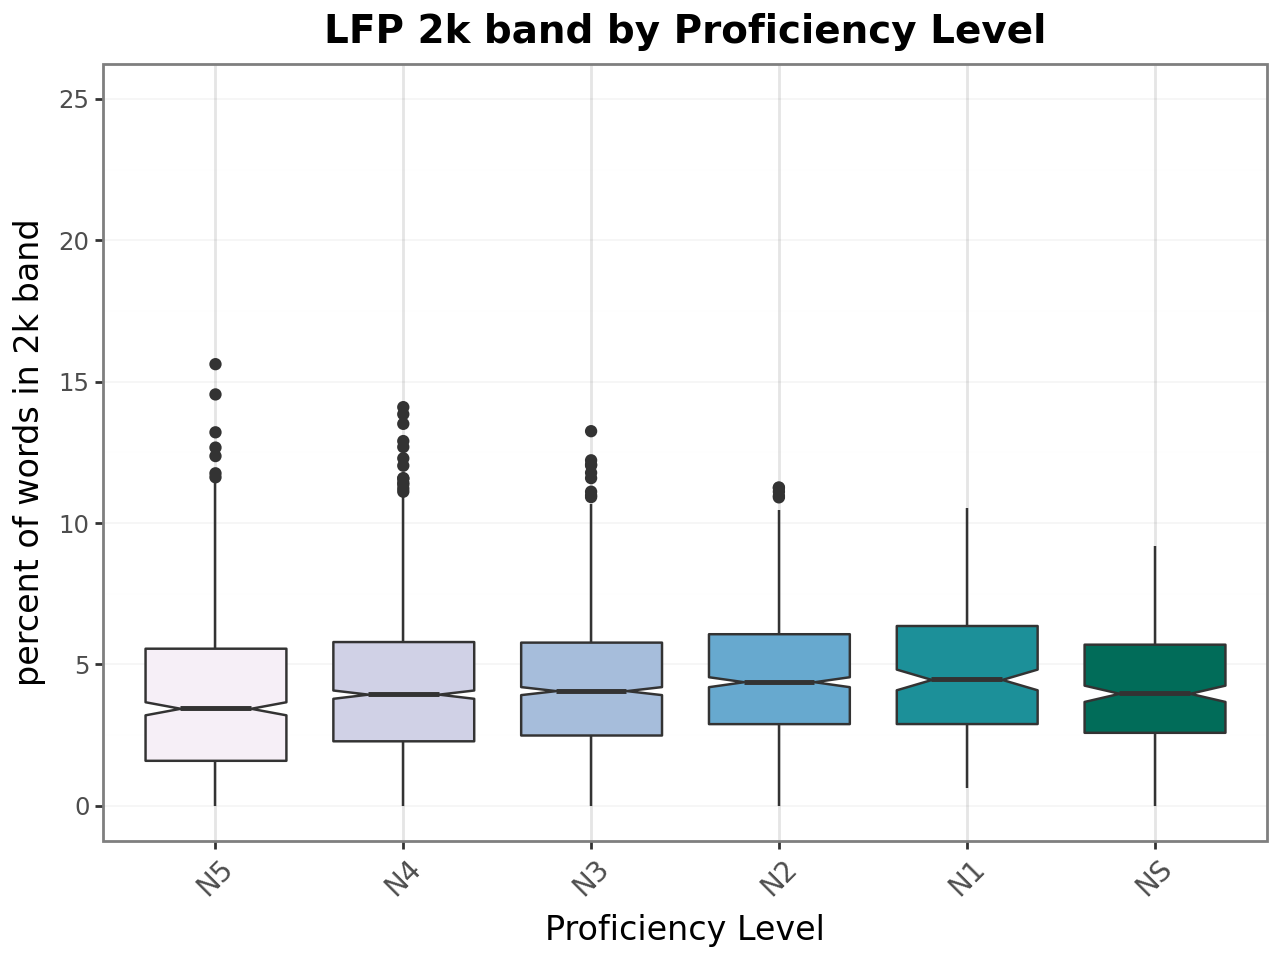
\includegraphics[scale=.4]{img/LFP/2k}
        \caption[Percentage of tokens used from 2k band]{}
\label{fig:2kband}
\end{minipage}
    \end{figure}


\begin{figure}[htbp]
    \centering
    \begin{minipage}{.48\textwidth}
        \centering
    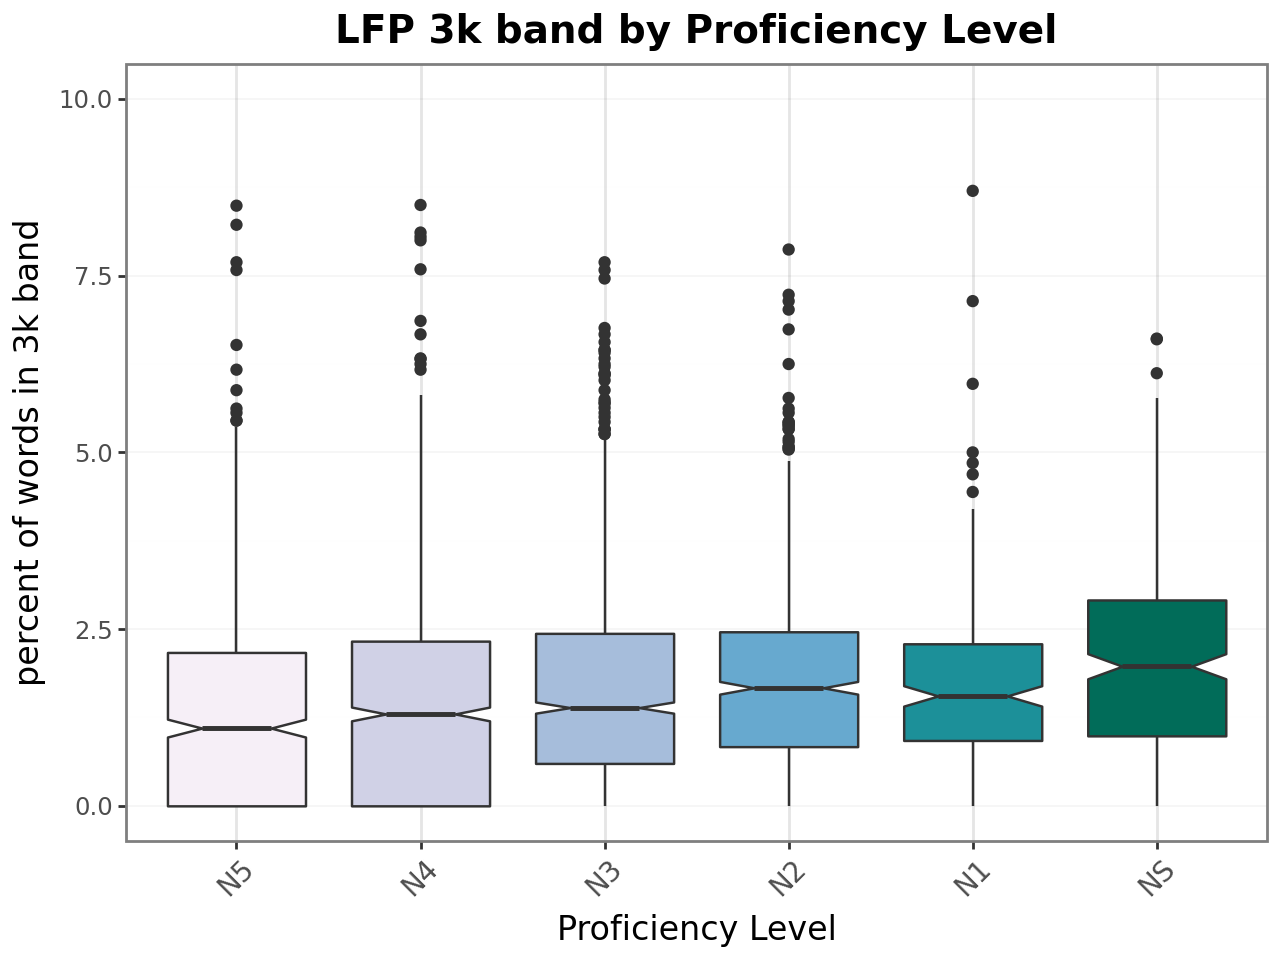
\includegraphics[scale=.4]{img/LFP/3k}
    \caption[Percentage of tokens used from 3k band]{}
        \label{fig:3kband}
    \end{minipage}
    \hfill
\begin{minipage}{.48\textwidth}
        \centering
        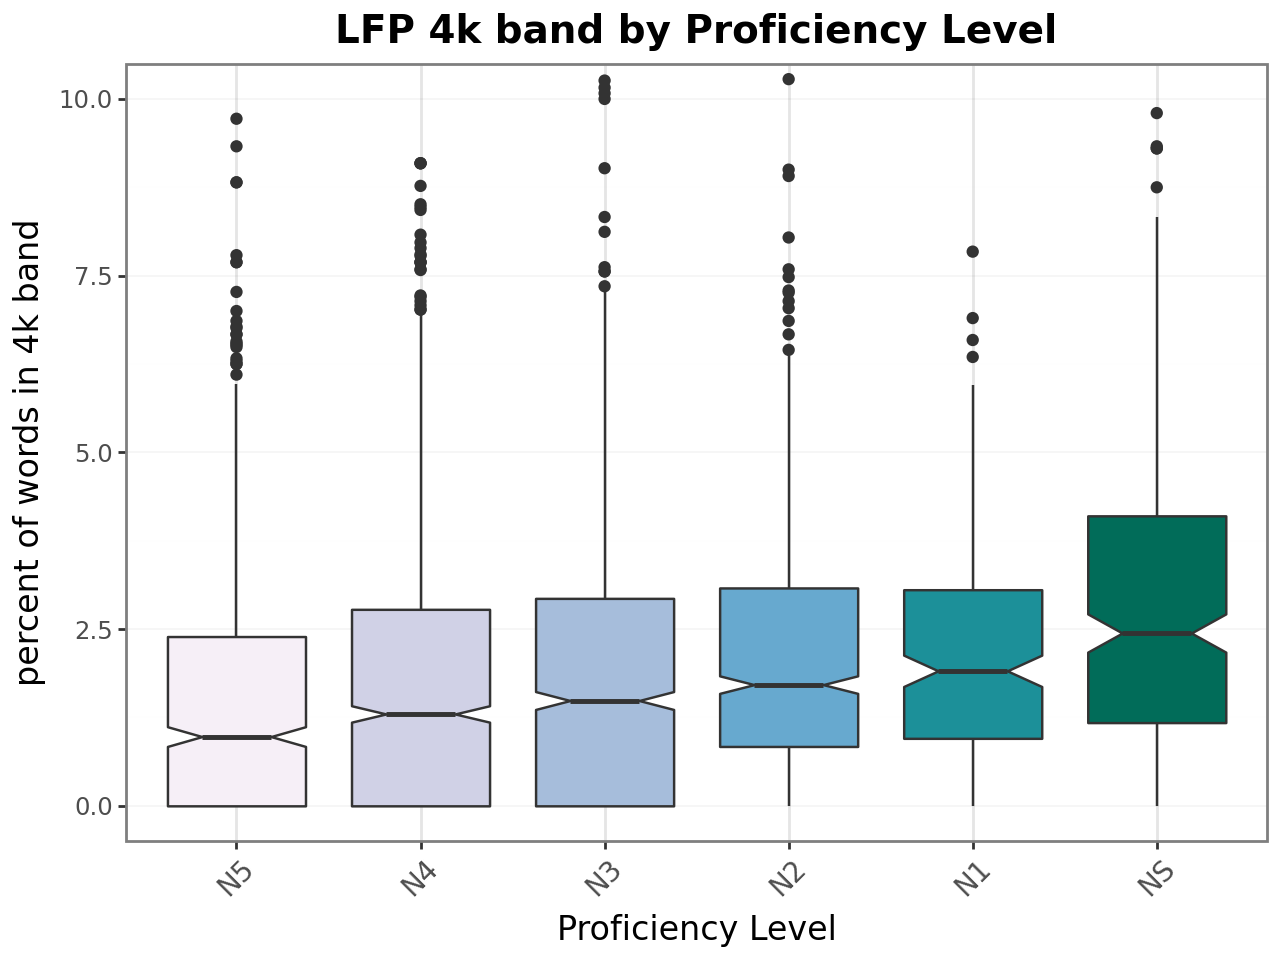
\includegraphics[scale=.4]{img/LFP/4k}
        \caption[Percentage of tokens used from 4k band]{}
\label{fig:4kband}
\end{minipage}
    \end{figure}

Out-of-Vocabulary (OOV) items also decreased with proficiency. Statistically significant
differences were found both at the lower (N5-N4,
N4-N3),
 proficiency levels. This measure was also able to distinguish between the N1 and native speaker(NS) group. This
suggests that lower-level learners may have used more off-list or erroneous forms, while more proficient speakers
had more controlled lexical output.



%LFP - JLPT WordList
    %*percentage of N5 words slightly decreases across proficiency levels to show higher learner's preference for
    %vocabulary from the higher lists (just like for the BCCJW).
    %N5- No statistical difference between the beginner-intermediate levels (N5-N3) then N3-N2 shows statistical
%significant different (meaning this can be used to differentiate between the beginning and advanced levels)

%N4 - increases across JLPT levels. Statistical significance between N5&N4 and N4&N3

%N3 - not noteable at all the vocabulary use at this level stayed flat and nothing was statistically significant.

%N2- Significant difference between all levels but the lower N5&N4. also increases across proficiency levels.

%N1 - statistical significance between N5&N4, N4&N3, but not at distinguishing the higher proficiency levels.\

An additional analysis was conducted using JLPT-aligned vocabulary lists. Results from this alternative
approach were broadly consistent with the BCCWJ-based findings. Words from the
N5 list were commonly used across all proficiency levels, but their relative frequency declined steadily as
proficiency increased.
While no statistically significant differences were found among the beginner groups (N5 to N3), a marked shift
was observed between
N3 and N2, indicating that N5 vocabulary use may help distinguish between beginner and advanced learners(
Figure~\ref{fig:JLPTN5vocab}).

N4 level vocabulary showed a gradual increase across levels peaking around N2, followed by a slight decline 
at N1(Figure~
\ref{fig:JLPTN4vocab})
. Statistically significant
differences were observed between N5 and N4 and
between N4 and N3. In contrast, N3 vocabulary use remained relatively flat across levels with no 
significant 
differences,
indicating that these words may not effectively distinguish between proficiency groups (Figure~\ref{fig:JLPTN3vocab}).

\begin{figure}[htbp]
    \centering
    \begin{minipage}{.48\textwidth}
        \centering
    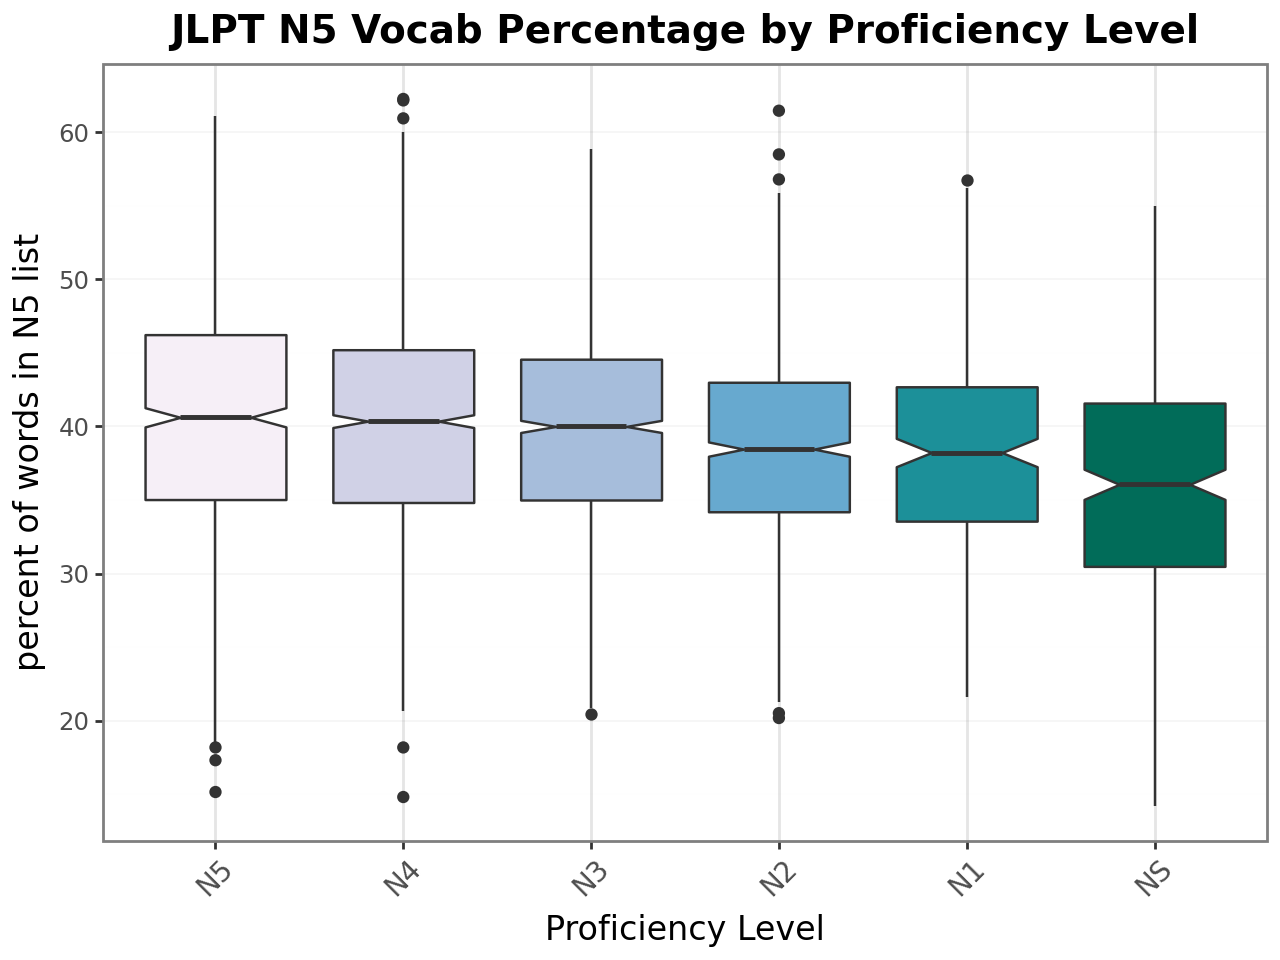
\includegraphics[scale=.4]{img/LFP/JLPT_N5}
    \caption[Percentage of tokens used from JLPT N5 List]{}
        \label{fig:JLPTN5vocab}
    \end{minipage}
    \hfill
\begin{minipage}{.48\textwidth}
        \centering
        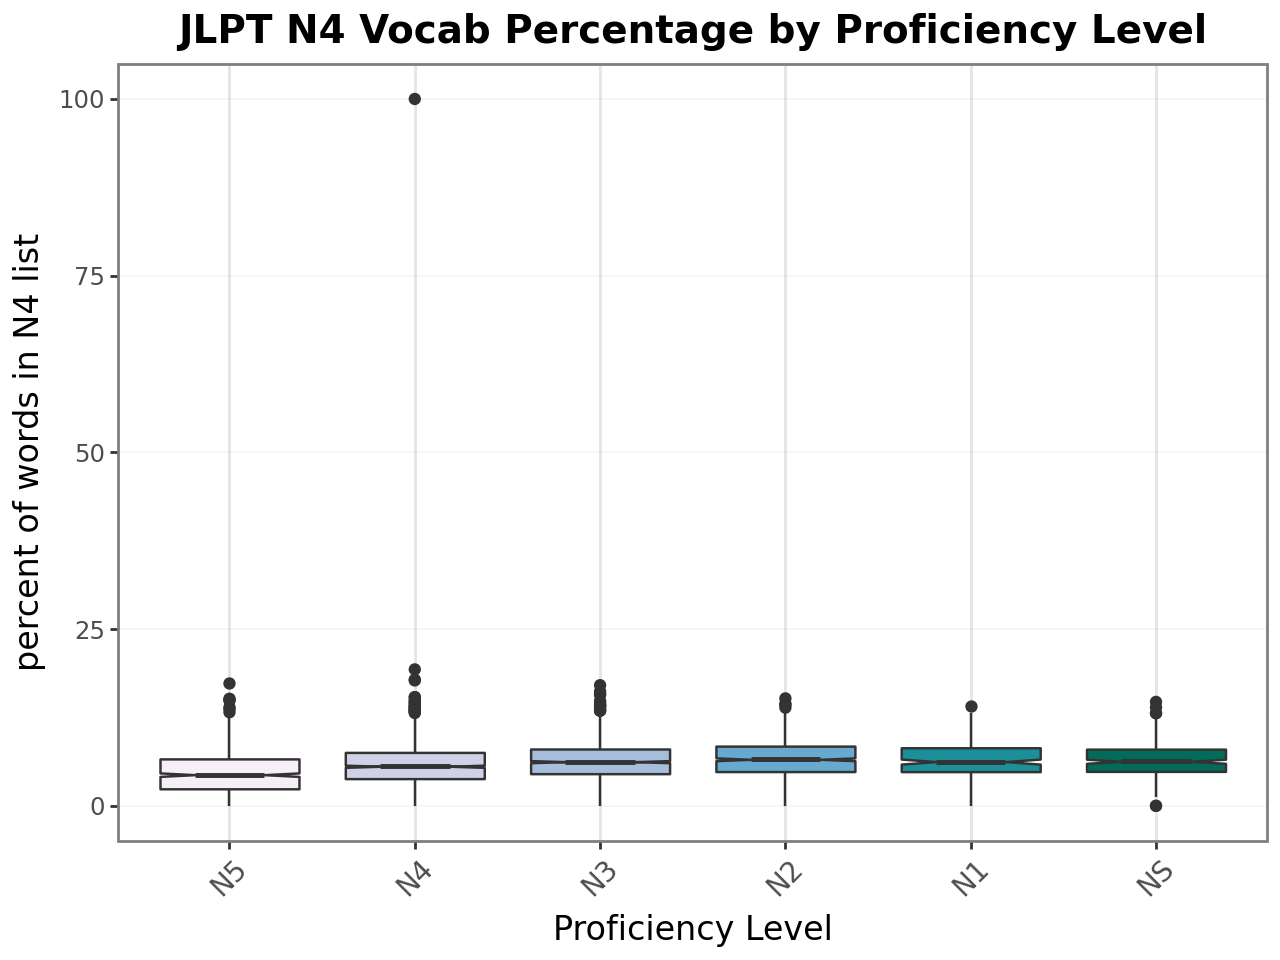
\includegraphics[scale=.4]{img/LFP/JLPT_N4}
        \caption[Percentage of tokens used from JLPT N4 List]{}
\label{fig:JLPTN4vocab}
\end{minipage}
    \end{figure}
N2 vocabulary, demonstrated consistent upward trajectory and significantly differentiated all levels
except the two lowest (N5 and N4) (Figure~\ref{fig:JLPTN2vocab}). Finally, N1 increased in useage but only showed 
significance at
distinguishing
the lower levels (N5-N4, N4-N3), and not between the more advanced groups (Figure~\ref{fig:JLPTN1vocab}). This 
may be due to the nature
of N1 vocabulary, which often include low-frequency or domain-specific terms that may not be easily elicited 
through the given writing tasks. 

\begin{figure}[htbp]
    \centering
    \begin{minipage}{.48\textwidth}
        \centering
    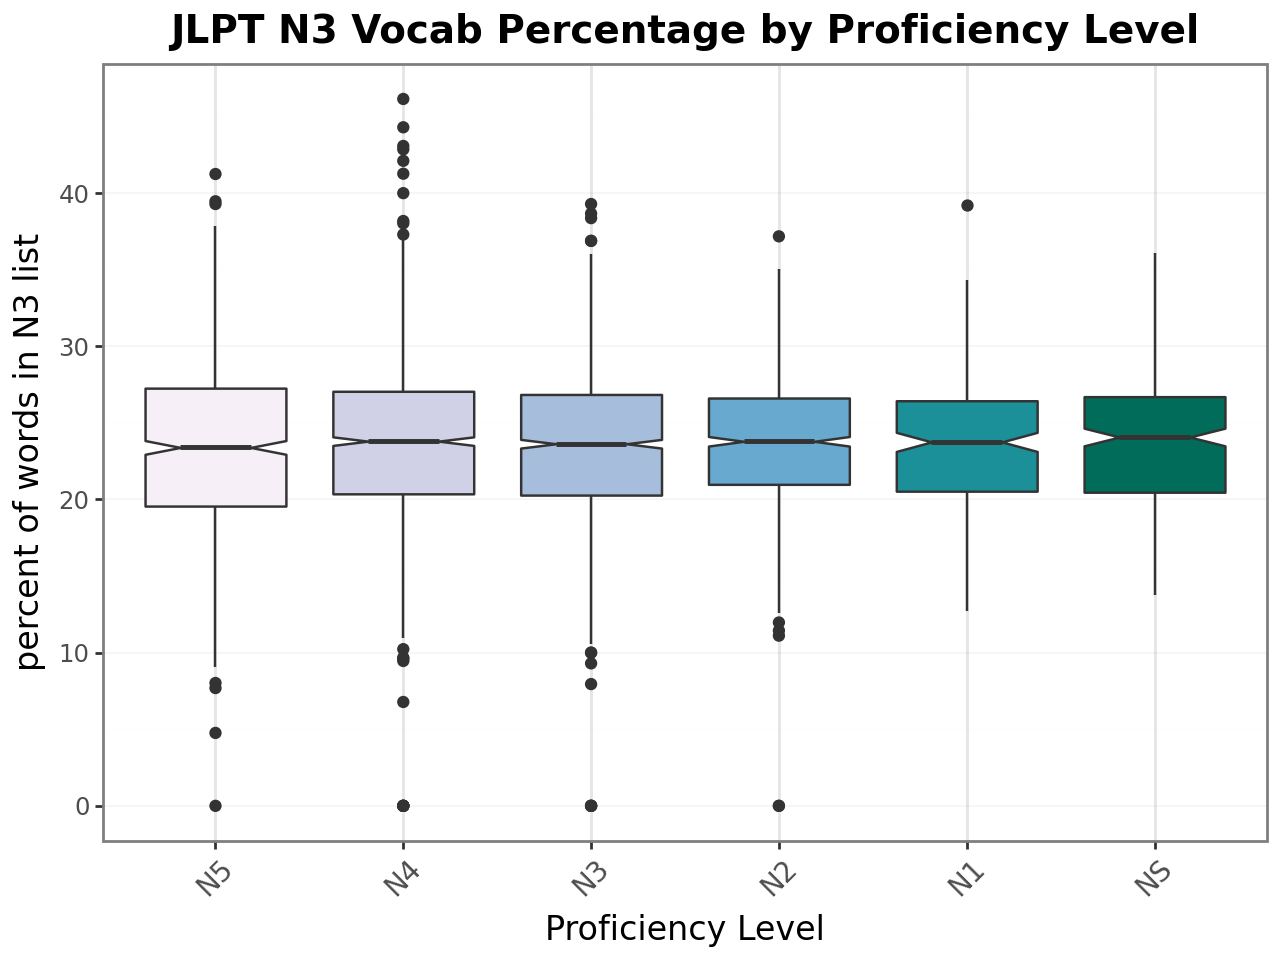
\includegraphics[scale=.4]{img/LFP/JLPT_N3}
    \caption[Percentage of tokens used from JLPT N3 List]{}
        \label{fig:JLPTN3vocab}
    \end{minipage}
    \hfill
\begin{minipage}{.48\textwidth}
        \centering
        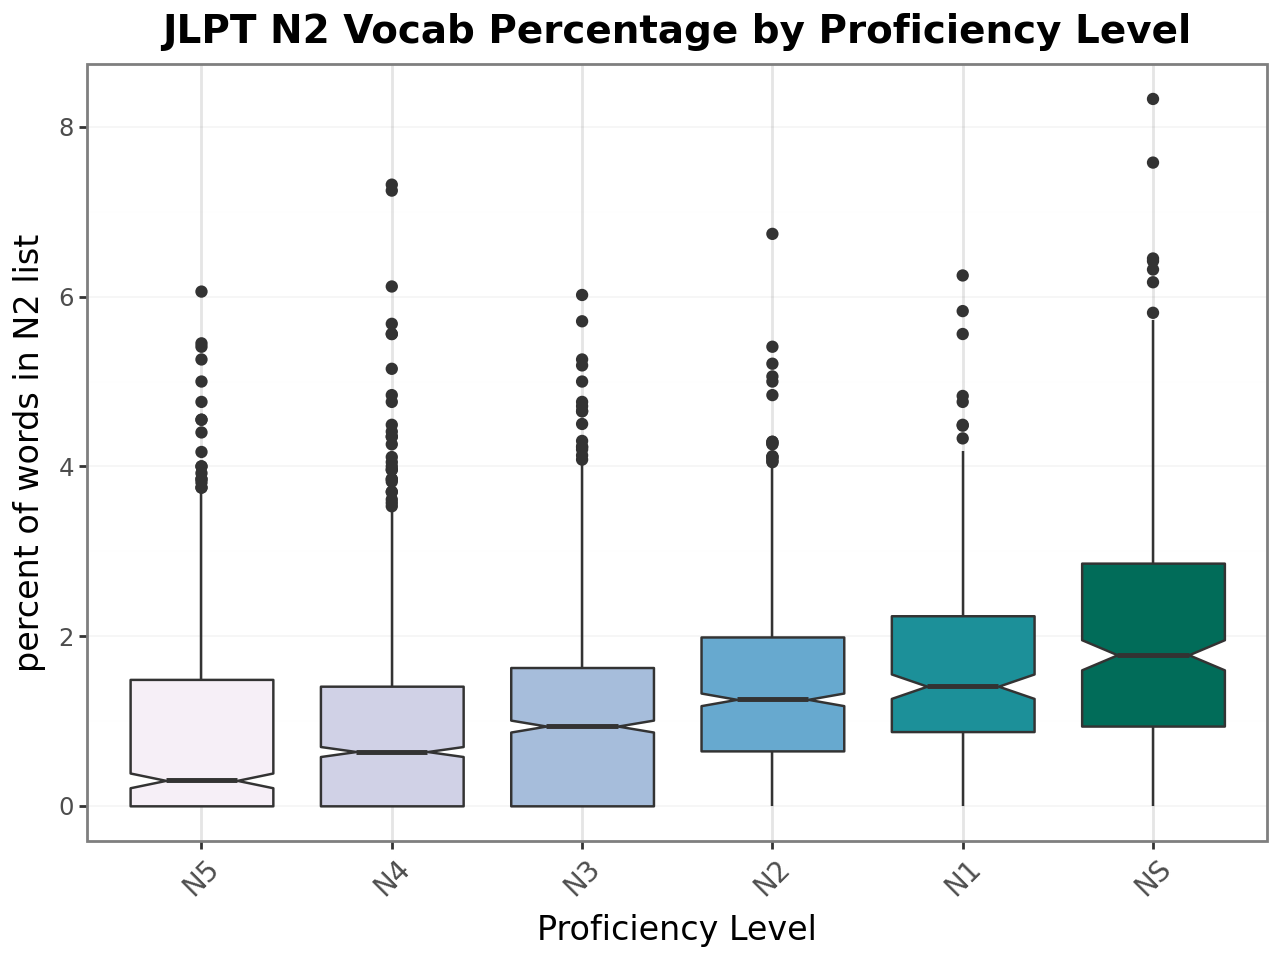
\includegraphics[scale=.4]{img/LFP/JLPT_N2}
        \caption[Percentage of tokens used from JLPT N2 List]{}
\label{fig:JLPTN2vocab}
\end{minipage}
    \end{figure}

\begin{figure}
           \centering
           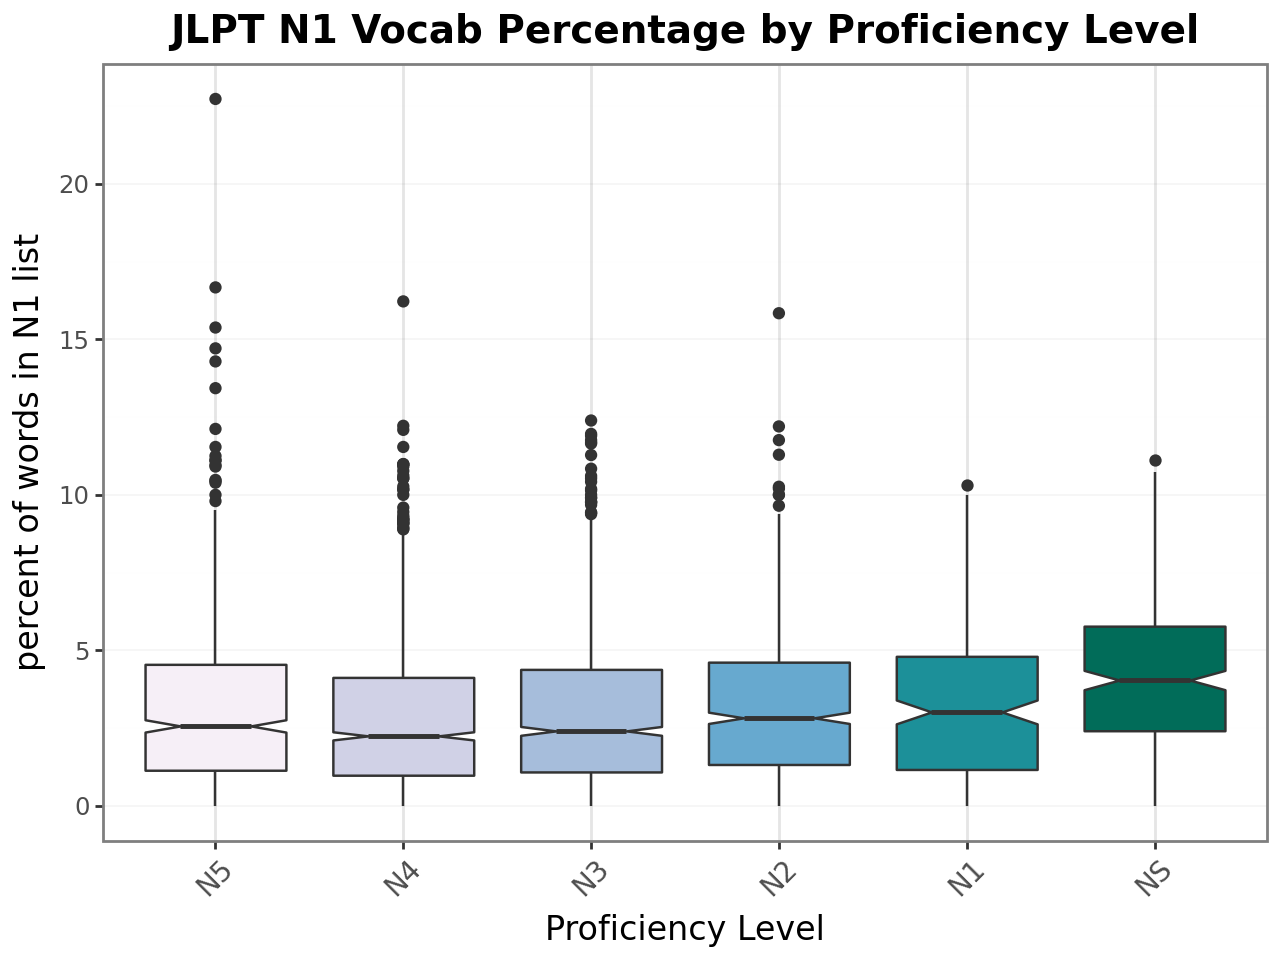
\includegraphics[scale=.5]{img/LFP/JLPT_N1}
           \caption{Percentage of tokens used from JLPT N1}
           \label{fig:JLPTN1vocab}
\end{figure}


\subsection{Morphological Complexity Measures}
This section reports on morphological complexity through two indices, the Morphological Complexity Index (MCI)
\citep{Brezina2019} and JRMA based on the Korean Readability Morphological Analyzer \citep{Hwang2024}. Thease
measures aim to observe how learners employ morphological elaboration, either through surface variation or content
and function word use.

\subsubsection{MCI Measures}

%MCI 5-Surface
%\begin{itemize}
%   \item *33 texts removed
%   \item  *Increase across levels
%    \item *statistically significant across groups except N1&NS and N1 and N2
% \end{itemize}

The Morphological Complexity Index was computed using both surface and inflectional types across two window sizes (
MCI-5 and MCI-10). For MCI-5 using surface forms 33 texts were excluded due to insufficient token count. A clear
increase in complexity was observed across proficiency levels, with statistically significant differences between
the most groups except N1-N2 (Figure~\ref{fig:MCI5surface}). This suggests that the measure is sensitive to early and
intermediate stages of
development
but plateaus among advanced learners.


\begin{figure}[htbp]
    \centering
    \begin{minipage}{.48\textwidth}
        \centering
    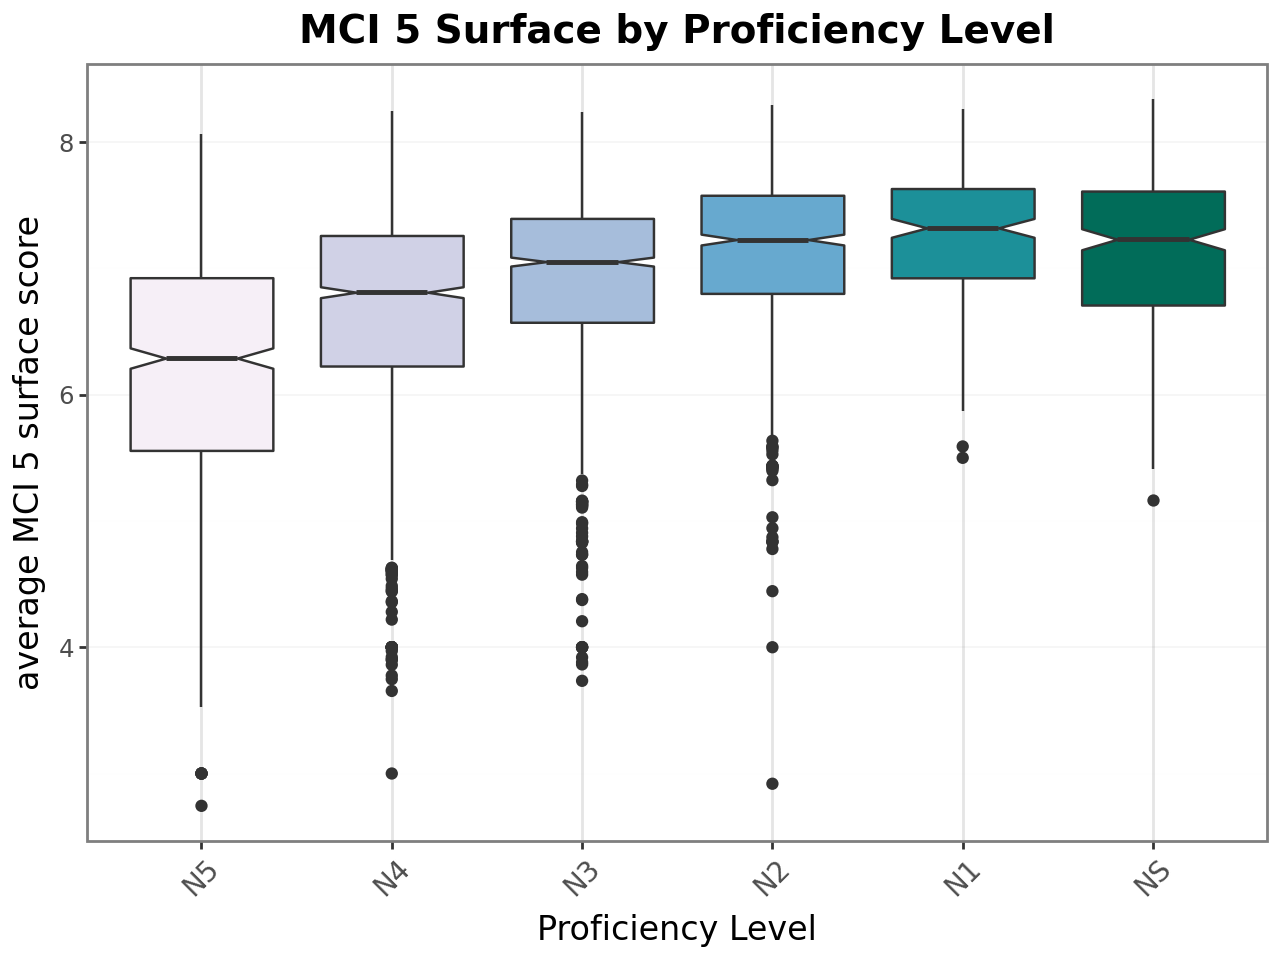
\includegraphics[scale=.4]{img/MCI5surface}
    \caption[MCI 5 surface scores across Proficiency levels]{}
        \label{fig:MCI5surface}
    \end{minipage}
    \hfill
\begin{minipage}{.48\textwidth}
        \centering
        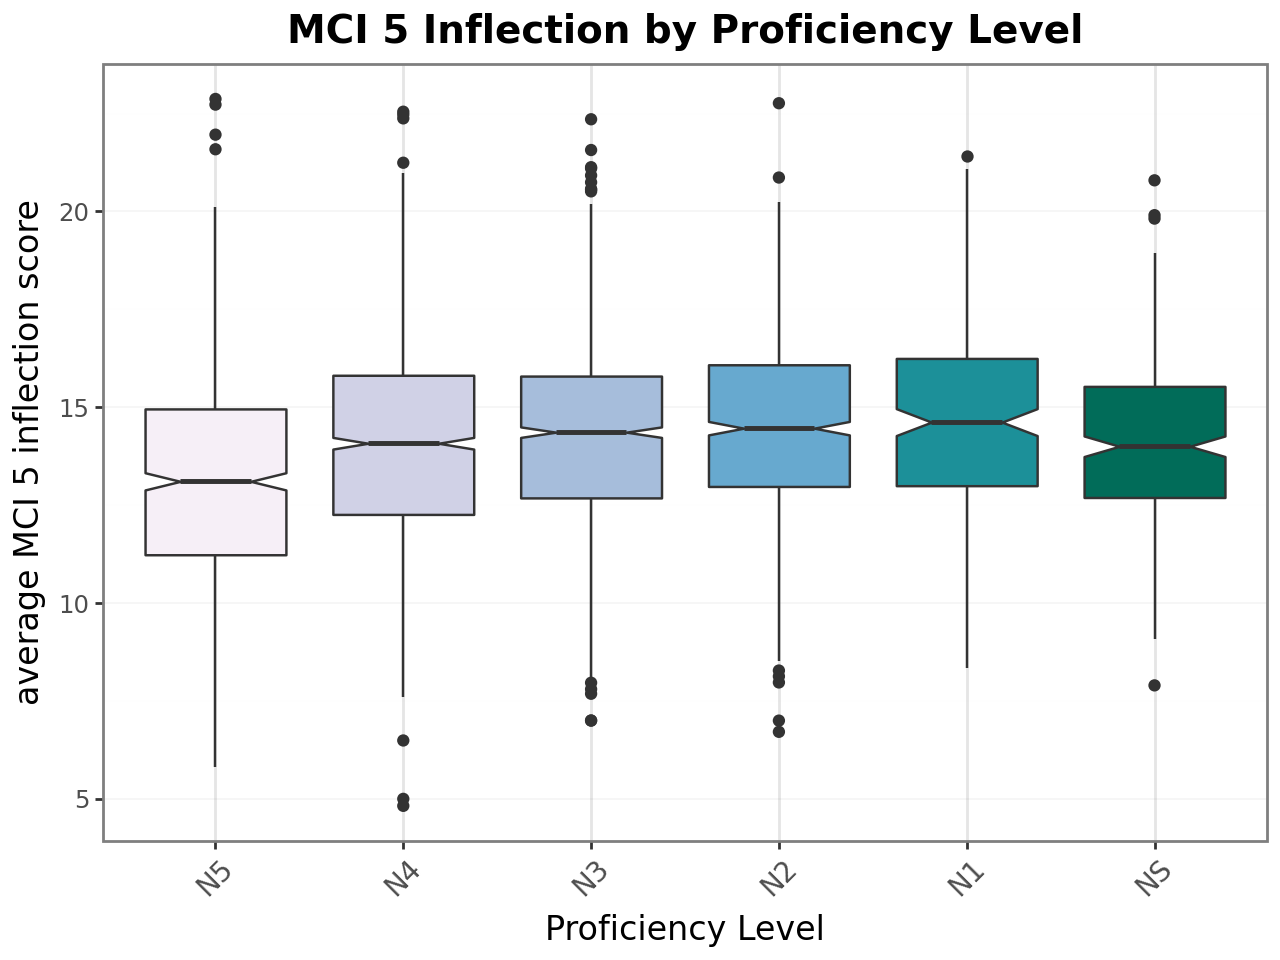
\includegraphics[scale=.4]{img/MCI5inflection}
        \caption[MCI 5 inflection scores across Proficiency levels]{}
\label{fig:MCI5inflection}
\end{minipage}
    \end{figure}

%MCI 5-Inflection
%    *33 texts dropped
%    *not as great an increase across levels
%    *does not discriminate between adjacent levels but every other level at lower levels N5&N3, N4&N2

In contrast, the inflection based MCI-5 measure showed a weaker overall trend(Figure~ref\{img/MCI5inflection}).
While is captured
statistically
significant differences between non-adjacent and lower-level pairs such as N5-N3 and N4-N2, it failed to distinguish
between adjacent levels, indicating lower sensitivity compared to the surface-based version.


%MCI 10 - Surface (621 texts dropped)
    %* Increase across levels
    %* Statistically significant at lower levels N5 - N2 , no significance between N2, N1, NS
%MCI 10 - Inflection
%    *statistically significant difference between N1 and NS!
%    *Statistically significant at lower levels N5-N2, no significance between N2 and N1

MCI-10 results mirror these trends but were more restrictive. Due to the larger window size, the surface-based MCI-10
required longer texts, leading to the exclusion of 621 samples due to low token count.  Despite this, it showed an
upward trend in complexity and statitically significant differences up to the N2 level (Figure~\ref{fig:MCI10surface}). However, no
differences were
observed among the highest levels, again indicating a ceiling effect. The inflection-based MCI-10 was the only
version that yielded a significant distinction between the N1 and native speaker groups, although its discriminatory
power was also limited to the lower levels otherwise(Figure~\ref{MCI10inflection}).


\begin{figure}[htbp]
    \centering
    \begin{minipage}{.48\textwidth}
        \centering
    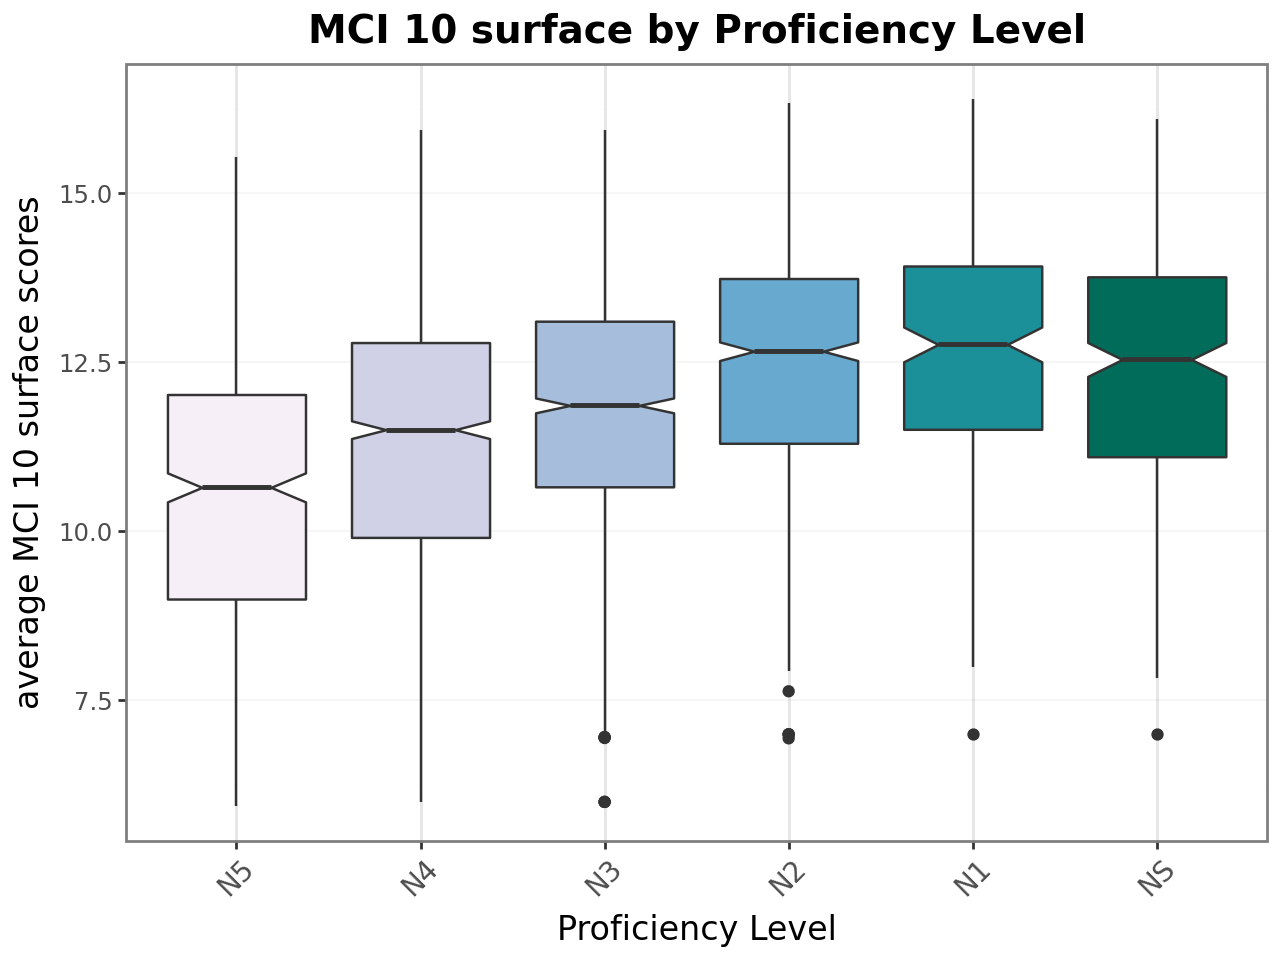
\includegraphics[scale=.4]{img/MCI10surface}
    \caption[MCI 10 surface scores across Proficiency levels]{}
        \label{fig:MCI10surface}
    \end{minipage}
    \hfill
\begin{minipage}{.48\textwidth}
        \centering
        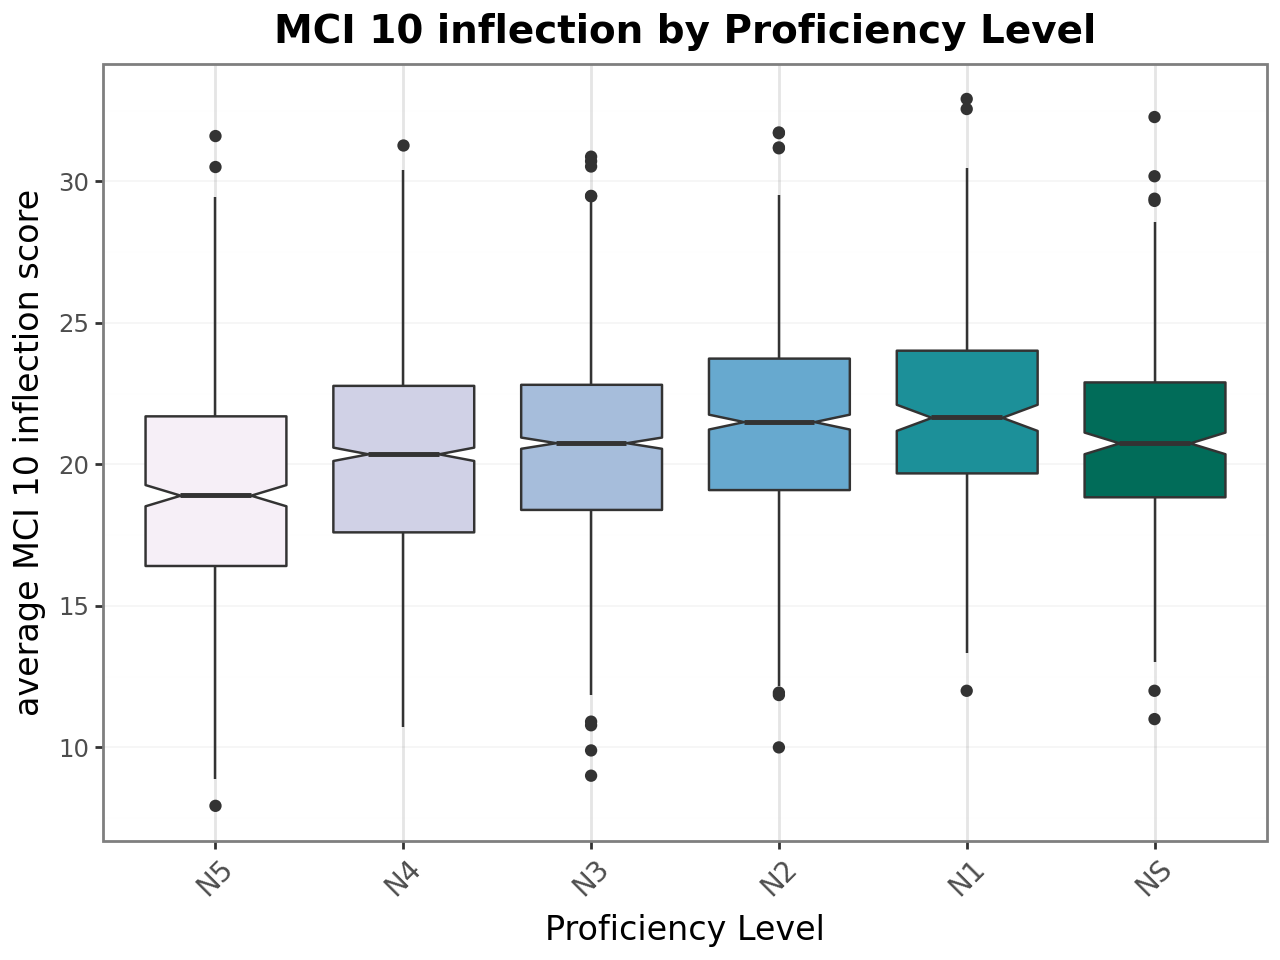
\includegraphics[scale=.4]{img/MCI10inflection}
        \caption[MCI 10 inflection scores across Proficiency levels]{}
\label{fig:MCI10inflection}
\end{minipage}
    \end{figure}

Overall, surface-based MCI-5 emerged as the most practical and sensitive measure, especially for lower proficiency
learners who are most likely to have shorter texts. It retains more data and yields strong significance patterns
without the dataloss issues introduced by MCI-10's longer window size requirement.

\subsubsection{JRMA-Based Measures}

%*MTLD measures had dropped texts due to the minimum text length limit required. This is especially true for
%these measures as it is using specific function/content words meaning even longer text is needed.
Morphological diversity was also evaluated using JRMA-based variants of MTLD and MATTR. Due to the structural
specificity of JRMA (focusing on functions vs. content words), these metrics has stricter text length requirements,
leading to large numbers of text exclusions.

\begin{figure}[htbp]
    \centering
    \begin{minipage}{.48\textwidth}
        \centering
    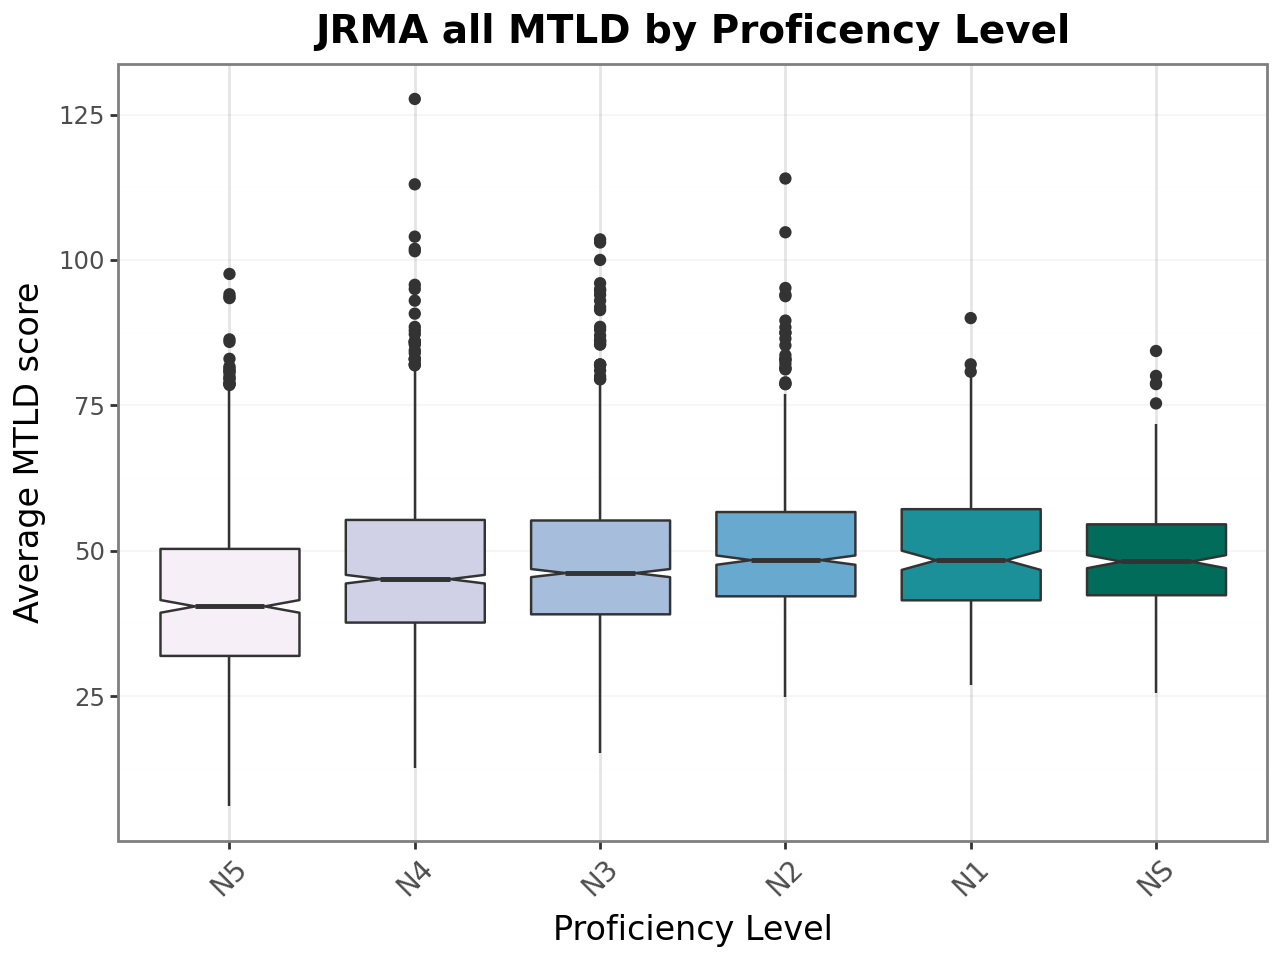
\includegraphics[scale=.4]{img/JRMA-MTLD-all}
    \caption[MTLD all]{}
        \label{fig:MTLDall}
    \end{minipage}
    \hfill
\begin{minipage}{.48\textwidth}
        \centering
        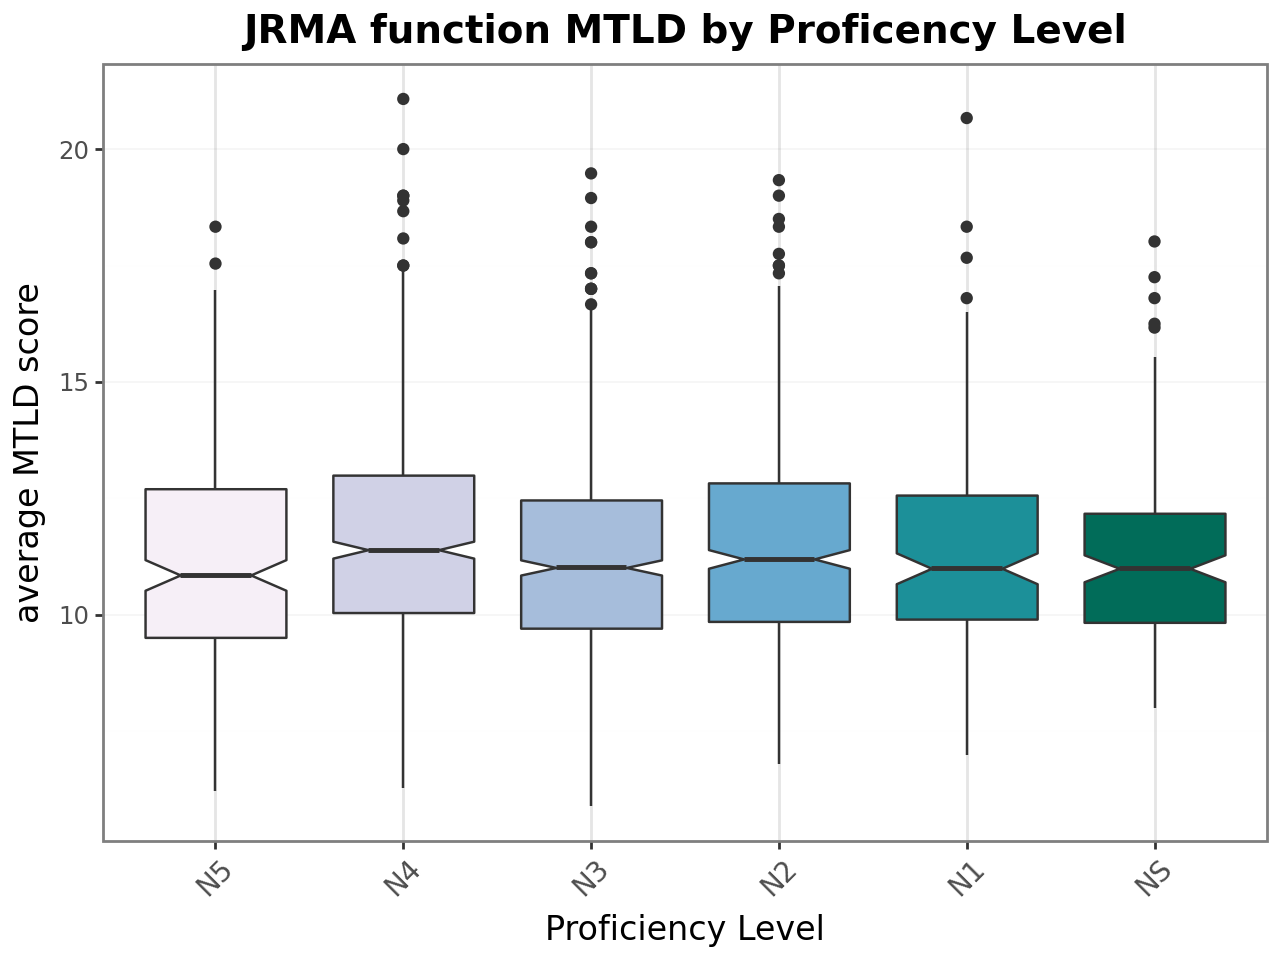
\includegraphics[scale=.4]{img/JRMA-MTLDfunction}
        \caption[MTLD Function]{}
\label{fig:MTLDfunction}
\end{minipage}
    \end{figure}
%JRMA_all_MTLD
   % *49 rows removed
    %*statistically significant difference in distinguishing N5&N4, N3&N2 levels

%JRMA_function_MTLD
    %*2365 rows removed
    %* only difference in N4 and N3 were statistically significant.
    %*no clear pattern of increasing/decreasing
%JRMA_content_MTLD
%    * 2433 rows removed of 4840
%    * Statistically significant in distinguishing the lower levels. N4&N5 N3&N2

For the JRMA MTLD calculation on the combined list of function and content words (JRMA_all_MTLD), 36 rows were removed
for not
meeting the minimum token length requirement. The measure successfully distinguished N5-N4 and N3-N2 non-adjacent
levels, with a
general upward trend (Figure~\ref{MTLDall}). However, the MTLD score for the function word list led to the removal of 2,
365
texts due to
text length, leading to weaker results (Figure~\ref{fig:MTLDfunction}). Consequently, only significance in
distinguishing
between N4-N3
levels was observed. No consistent developmental pattern was observed. Content-based MTLD required even longer
texts, excluding 2,433 texts (close to half of texts). Nevertheless, it captured meaningful differences at the lower 
levels in distinguishing between N5-N4 and N3-N2 levels(Figure~\ref{fig:MTLDcontent}). 


\begin{figure}[htbp]
    \centering
    \begin{minipage}{.48\textwidth}
        \centering
    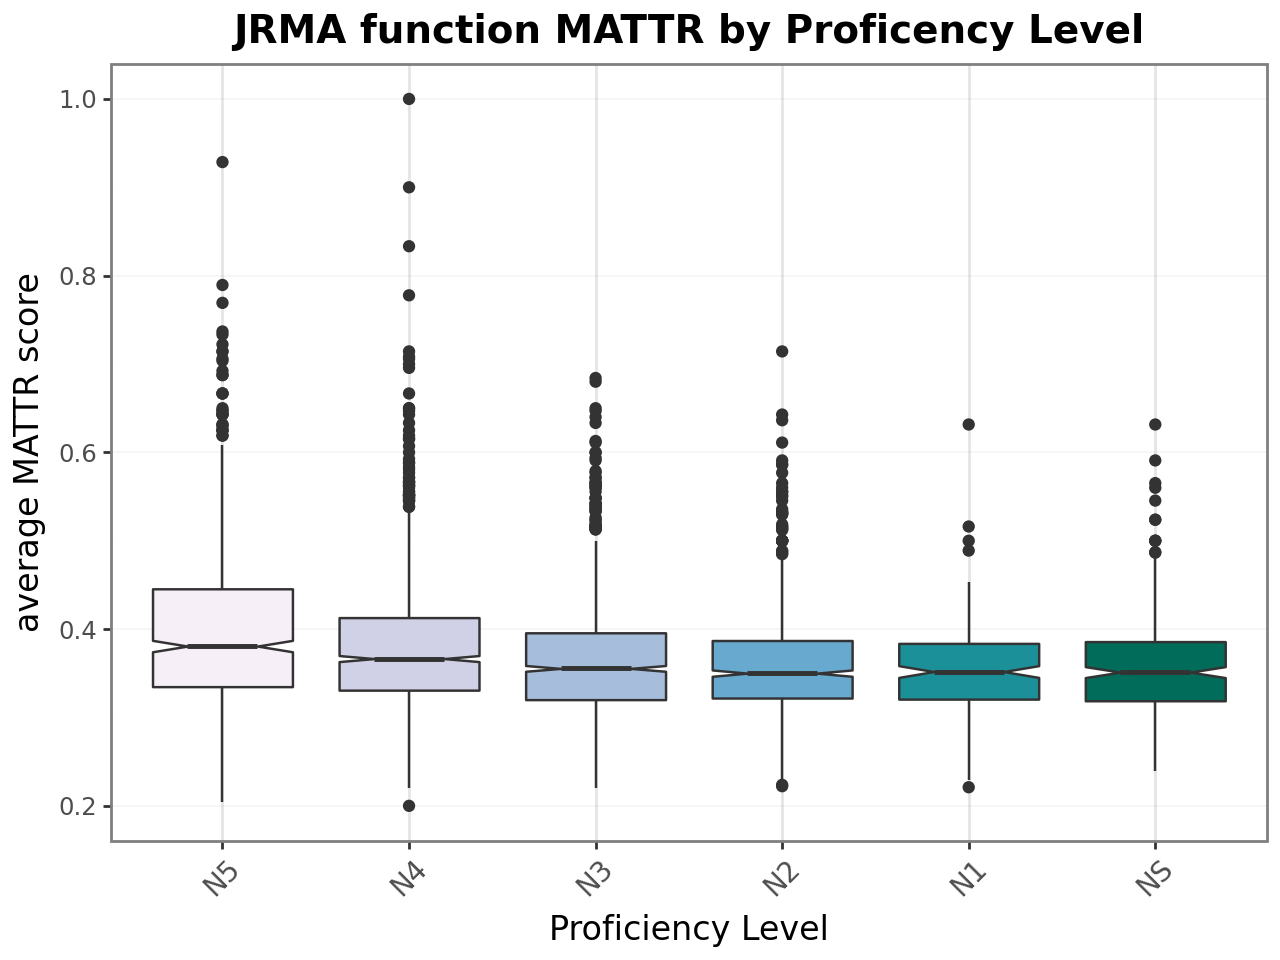
\includegraphics[scale=.4]{img/JRMA-MATTRfunction}
    \caption[MATTR function]{}
        \label{fig:MATTRfunction}
    \end{minipage}
    \hfill
\begin{minipage}{.48\textwidth}
        \centering
        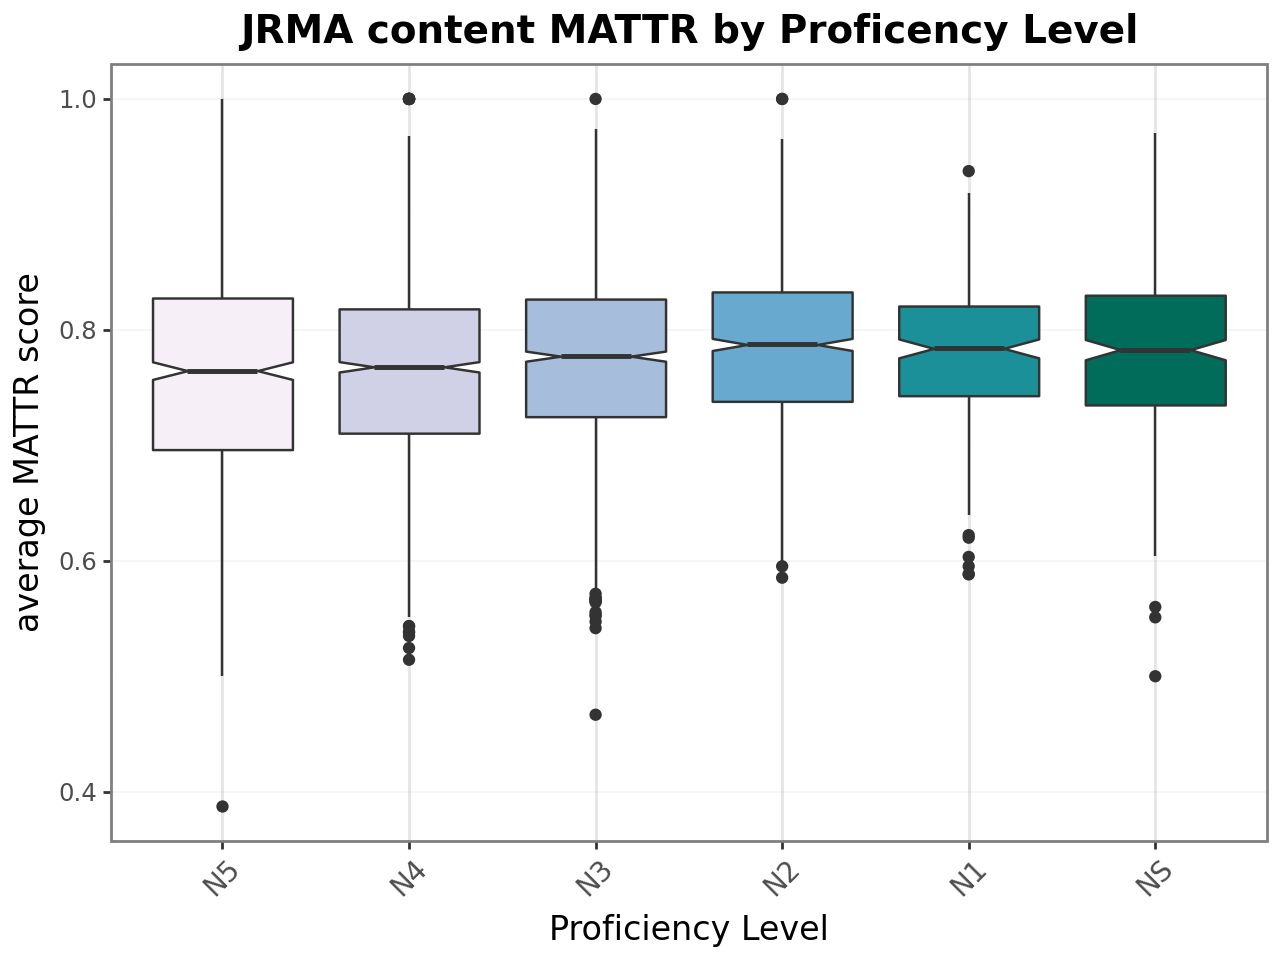
\includegraphics[scale=.4]{img/JRMA-MATTRcontent}
        \caption[MATTR content]{}
\label{fig:MATTRcontent}
\end{minipage}
    \end{figure}



%JRMA_all_MATTR
    %*Significant difference between all levels except the N1&NS,and N1&N2
    %* slight increase across levels, variance also decreases

%JRMA_Function_MATTR
    %*Slight decrease across levels.
    %*decrease in variance across levels
    %* significant pairs: (N5,N4), (N4,N3),(N5,N3)

%JRMA_Content_MATTR
    %* decrease in variance across levels
    %* significant pairs: (N2,N3), (N5,N3)

For the MATTR-based variants, the combined list of function and content words showed a slight increase in diversity
and a reduction in variance across proficiency levels. It yielded statistically significant differences between all
levels except N1-N2 (Figure~\ref{fig:MATTRall}). Function-based MATTR showed a slight decrease in diversity and
variance, distinguishing N5-N4, and N4-N3 levels (Figure~\ref{fig:MATTRfunction}). Content-based MATTR exhibited a
similar decline in variance and showed significant contrasts for N5-N3 and N3-N2 (Function~\ref{fig:MATTRcontent}).

\begin{figure}[htpb]
\centering
\includegraphics[scale=.5]{img/auxchains}
\caption[Average Length of auxilary verb chains]{}
\label{fig:auxchain}
\end{figure}
%Auxiliary Chains
    %* significant pairs (N5,N4),(N3,N5)
    %* increase from N5 to N4, but after that plateaus. Meaning that after the beginning levels chain size doesn't
    %increase
Lastly, auxiliary chain length was explored as a local morphological measure. It revealed a significant increase
from N5 to N4, but plateaued afterward (Figure~\ref{fig:auxchain}), suggesting that auxiliary chaining develops
primarily
at he
initial stages
and stabilizes among intermediate and advanced learners.


\subsection{Summary}
%Write here summarizing the most demonstrative complexity measures:
%i.e. Syntactic: Sent Length,Coordinate Clauses per sentence,  MDD, MHD
%Lexical: CTTR over MTLD? BCCJW corpus or JLPT wordlist? I'm not sure.
%Morphological: MCI5-surface, MATTR-all (combined function and content word list)
Several complexity measures stood out as particularly effective in capturing developmental trends across JLPT
proficiency levels.
From a syntactic standpoint, sentence length, coordinate clauses per sentences, and both Mean Dependency Distance (
MDD) and Mean Hierarchical Distance (MHD) consistently reflected increasing structural complexity. These measures
reliably distinguished between adjacent levels, especially in the intermediate to advanced range.

For lexical complexity, CTTR was sensitive to development at lower levels but plateaued later. While MTLD is
theoretically robust, its utility was limited due to text-length constraints. The BCCWJ-based Lexical Frequency
Profile proved more informative than the JLPT wordlist, especially in showing shifts in vocabulary distribution
across the 1k-4k bands.

In terms of morphological complexity, the MCI-5 surface form index was the most practical and sensitive measure,
avoiding the data loss seen with MCI-10 while still capturing developmental patterns. JRMA all-MATTR, combining both
ufnction and content word diversity, also showed a clear progression across levels and offered a stable profile of
lexical variation.

Overall, sentence length, coordinate clauses per sentence, MDD/MHD, CTTR, BCCWJ-based LFP, MCI-5 surface, and JRMA
all-MATTR were the most reliable indicators of linguistic development.

\section{Criterial Features}

%look at how many of structures from each level are used across all features used, just as was observed in \citet{
%akef2025} frequencies of the individual forms was low possibly due to stylistic choice or avoidance due to
%unfamiliarity etc.

%Due to the large amount of 0 in the data a Kruskal-wallis test and then Dunn's was run to analyze significance
%between pairs.

%In terms of development, N5 learners used 「~たい」(tai, to express desire to do something) the most, N4 learners also
%increasingly used 「~たい」 then from N3 and onwards the passive form (受身形, Ukemikei) is used increasingly across
%levels.

%Ukemi use increases across levels, Tai is used more frequently in the beginning levels and use decreases in N2 and
%N1, Tekuru use also increases across levels used most frequently by the Native speaker group. Tara plateaus at N3.
%Toomou peaks at N4 and then begins to decrease in the higher proficiency levels.

%tai with kruskal willis found to be nonsignificant, other grammar points were found to be significant (p<.005)


To examine the developmental trajectory of specific grammar forms, several JLPT aligned grammar forms were tracked
across proficiency levels.  As was also observed in \citet{akef2025}, the absolute frequencies of individual grammar
forms was relatively low, likely due to individual stylistic preferences, avoidance strategies, or incomplete
acquisition.

Table~\ref{tab:CF-form-freq} and Table~\ref{tab:CF-form-freq-ratio} provide further context on the overall
prevalence and normalized frequencies of grammar forms in the I-JAS Corpus.


\begin{table}[h!]
\centering
\begin{tabular}{ccc}
\hline \textbf{Form} & \textbf{\# JLPT Level} & \textbf{Raw Count} \\ \hline
受身形 (ukemi; passive)                & N4 & 2529 \\
〜たい (tai; desire)                  & N5 & 2156 \\
〜と思う (to omou; to think)          & N4 & 1981 \\
〜という (to iu; to quote)            & N3 & 1389 \\
〜たら (tara; conditional)            & N4 & 1330 \\
〜ように (youni; so that/in order to) & N4 & 948 \\
〜てくる (tekuru; aspectual)          & N4 & 926 \\
〜させる (saseru; causative)          & N4 & 555 \\
〜てください (tekudasai; request)     & N5 & 533 \\
〜たびに (tabini; each time)          & N3 & 527 \\
\hline
\end{tabular}
\caption[Raw frequency of Top 10 Forms extracted from the I-JAS Corpus]{The raw count of the top 10 forms extracted
from the learner texts}
\label{tab:CF-form-freq}
\end{table}

\begin{table}[h!]
\centering
\begin{tabular}{ccc}
\hline \textbf{Form} & \textbf{\# JLPT Level} & \textbf{Ratio} \\ \hline
〜たい (tai; desire)                      & N5 & 0.00285 \\
受身形 (ukemi; passive)                  & N4 & 0.00270 \\
〜と思う (to omou; to think)             & N4 & 0.00201 \\
〜たら (tara; conditional)               & N4 & 0.00158 \\
〜てくる (tekuru; aspectual)             & N4 & 0.00126 \\
〜という (to iu; to quote)               & N3 & 0.00121 \\
〜ように (youni; so that/in order to)    & N4 & 0.00078 \\
〜てください (tekudasai; request)        & N5 & 0.00066 \\
〜させる (saseru; causative)             & N4 & 0.00065 \\
〜つもり (tsumori; intention)            & N5 & 0.00058 \\
\hline
\end{tabular}
\caption[Top 10 Grammar forms by normalized token ratio extracted from the I-JAS Corpus]{Normalized frequency of top
10 grammar forms. Normalization was done with the ratio of form to token count to control for text length. }
\label{tab:CF-form-freq-ratio}
\end{table}


To account for differences in text length, all grammar forms were normalized by token count (i.e., form-to-token
ratio). Given the large number of zeros values, non-parametric tests were used. Kruskal-Wallis
tests identified overall group-level effects, followed by Dunn's post hoc comparison for pairwise significance testing.


Five grammar forms were selected for closer analysis based on their frequency and theoretical relevance:

\begin{itemize}
\item \textbf{「〜たい」}(N5) - \textit{tai}, used to express desire.
\item \textbf{「〜たら」}(N4) - \textit{tara}, conditional clause marker.
\item \textbf{「〜てくる」}(N4) - \textit{tekuru}, aspectual or completive form.
\item \textbf{「〜とおもう」}(N5) - \textit{to omou}, expressing thoughts or uncertainty.
\item \textbf{受身形}(N5) - \textit{ukemikei}, the passive form.
\end{itemize}

A general line plot showing the useage ratio of each of the above grammar forms across levels is shown in
Figure~\ref{fig:CF-plot}. It can be seen that certain proficiency groups use different forms more frequently in
their writing.

\begin{figure}[h]
\centering
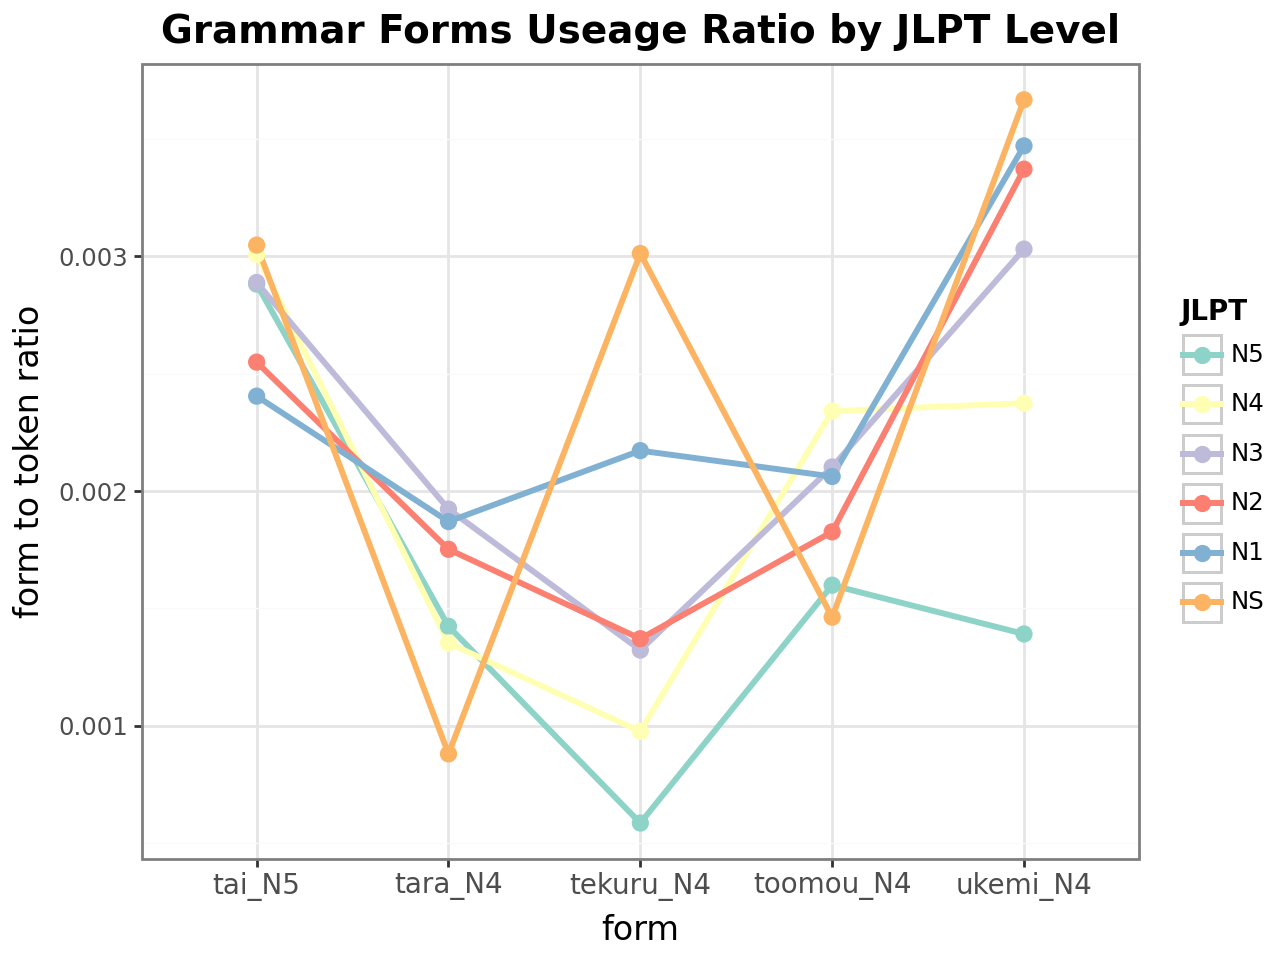
\includegraphics[scale=.5]{img/CF-plot}
\caption[The use of the top 5 frequently used grammar forms across JLPT levels]{}
\label{fig:CFplot}
\end{figure}


Among beginner learners (N5 and N4), 「〜たい」(tai) was the most frequently used form. Its use gradually declined with
increasing proficiency and was not statistically significant across groups($p$=0.5821), as confirmed by the lack of
significant p-values in Figure~\ref{fig:CFheatmap} for any pairwise comparison involving thie form. This suggests that
while used by beginners, it does not serve as a strong discriminator for developmental stages.


\begin{figure}[h!]
\centering
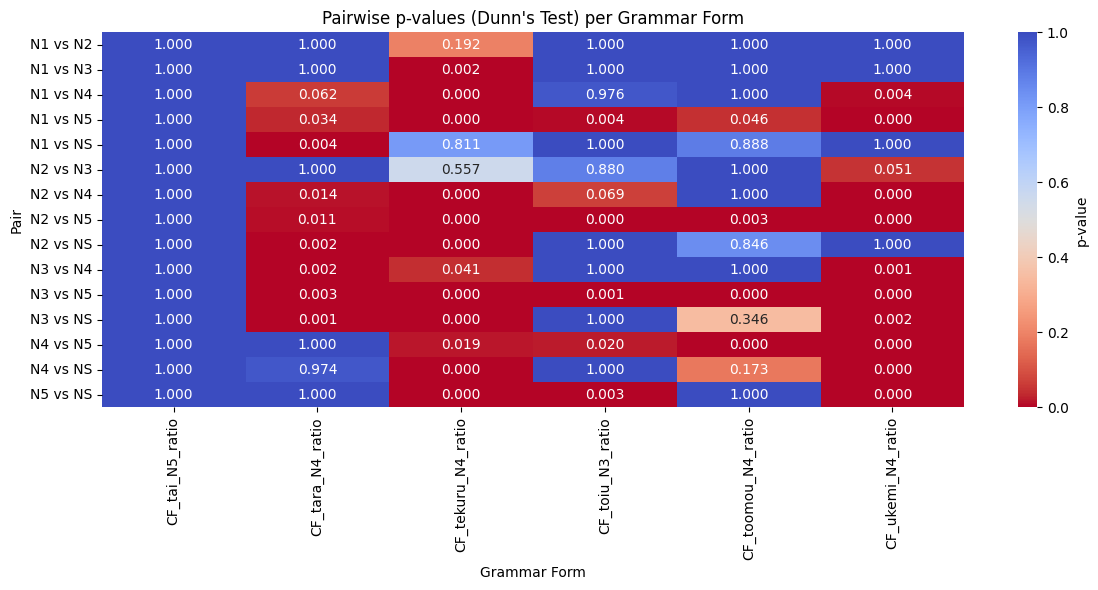
\includegraphics[scale=.4]{img/CFheatmap}
\caption[Heatmap of top 5 grammar forms]{}
\label{fig:CFheatmap}
\end{figure}

In
contrast, the
passive form (受身形) showed a clear upward trend in usage across proficiency levels. It was statistically significant
across many level comparisons ($p$<.001), including N5-N4, N4-N3, N4-N2, as indicated in Figure~\ref{fig:CFheatmap}.
This suggest strong potential as a critical feature for tracking development in the lower to intermediate
proficiency ranges. However, its developmental signal appeard to flatten at higher levels, as it was not significant
between certain adjacent levels(e.g. N3-N2, N2-N1). Nonetheless, the effect sizes observed between beginner
and advanced groups underscore its value in capturing major developmental differences.

「〜てくる」(tekuru) showed a steady increase in frequency across proficiency levels, and was used most by the native speaker
group. It was
statistically significant across almost all JLPT levels, as shown by the significant p-values for most pairings in
Figure~\ref{CFheatmap}. Exceptions included N2-N1 and N2-N2, indicating a possible plateau or more nuanced
development at the higher intermediate to advanced stages.


The usage of 「〜とおもう」 (to omou) peaked at the N4 level, followed by a noticeable decline in the higher proficiency
groups. Its
use was
significant across most pairings up to N1 as shown in Figure~\ref{fig:CFheatmap}. This pattern might reflect its
transitional
role, perhaps being a common early strategy for expressing
internal states or
opinions before learners acquire a wider range of more nuanced expressions.

The conditional marker,「〜たら」(tara) appeared to plateau  around the intermediate levels (
N3). Despite this, it was still statistically significant across several adjacent groups, including N5-N3 and N4-N2,
as indicated by the significant p-values in Figure~\ref{fig:CFheatmap}. This suggests its utility in discriminating
between certain non-adjacent or adjacent lower-to-mid proficiency levels.

%Talk about this chart and how Tekudasai only appears at the beginner level N5 and that the causative form appears at
%N1. integrate into the rest of the section so it isn't redundant.....
In Table~\ref{tab:CF-top6-per-level} a granular view of how the normalized usage of specific grammar forms changes
across each proficiency level is presented. The table highlights that 「〜てください」(tekudasai), a common polite request,
appears exclusively at the N5 (beginner) level in this selection with no presence in the higher levels. This
suggests it as a feature of early-stage production. Similarly, 「〜たい」(tai) shows its highest usage in N5 and N4,
gradually decreasing, reinforcing its usefulness as a idex of beginner-level development.

The passive form shows a clear progressive increase in ratio from N5 all the way to the native speaker group,
supporting
its
rule as a strong developmental marker. 「〜てくる」(tekuru) also exhibits a notable increase, especially from N3 (.00132)
to N1 (.00217), indicating its continued development into advanced stages. 「〜という」(toiu) also shows a gradual
increase from N5 to N1.

「〜とおもう」(to omou) peaks at N4 (.00234) and then shows a slight decline, aligning with the earlier observation of its
potential transitional role. 「〜たら」(tara) demonstrates a more stable presence across intermediate levels (N4-N1),
with its absence for the NS group being notable in this specific sample.

The causative form 「〜させる」(saseru) is notably absent from N5 to N2 and appears only at the N1 and Ns levels, with its
highest ratio in the NS group. This suggests it as a marker of high proficiency acquisition, reflecting the
complexity of causative constructions.

\begin{table}[h!]
\centering
\small
\resizebox{\textwidth}{!}{
\begin{tabular}{>{\raggedright\arraybackslash}m{3.5cm}lcccc}
\hline
\textbf{Form} & \textbf{N5} & \textbf{N4} & \textbf{N3} & \textbf{N2} & \textbf{N1} & \textbf{NS} \\
\hline
〜たい (tai)\\ \textit{desire} & 0.00288 & 0.00301 & 0.00289 & 0.00255 & 0.00240 & 0.00305 \\
〜と思う (to omou) \\ \textit{to think} & 0.00160 & 0.00234 & 0.00210 & 0.00183 & 0.00206 & 0.00146 \\
〜たら (tara)\\ conditional & 0.00142 & 0.00135 & 0.00192 & 0.00175 & 0.00187 & --- \\
受身形(ukemi)\\ passive & 0.00139 & 0.00237 & 0.00303 & 0.00337 & 0.00347 & 0.00367 \\
〜という (to iu)\\ \textit{to quote} & 0.00105 & 0.00115 & 0.00120 & 0.00133 & 0.00145 & 0.00142 \\
〜てくる (tekuru)\\ aspectual & --- & 0.00098 & 0.00132 & 0.00137 & 0.00217 & 0.00301 \\
〜てください (tekudasai)\\ polite request) & 0.00084 & --- & --- & --- & --- & --- \\
〜させる (saseru)\\ causative & --- & --- & --- & --- & --- & 0.00121 \\
\hline
\end{tabular}
}
\caption{Top Grammar Forms by Ratio Across JLPT Levels (Top 6 per level)}
\label{tab:CF-top6-per-level}
\end{table}



\subsection{Summary}
Overall, while the frequency of many individual forms remains relatively low, their distinct developmental trajectories
suggest potential as
criterial features. Particularly the passive form (受身形) and 「〜てくる」(tekuru) emerge as particularly strong candidates
for tracking proficiency development due to their consistent upward trends and widespread statistical significane
across multiple proficiency level comparisons.

%should I also mention the limitation of the tasks? certain tasks ellicit certain forms...
One limitation of
this analysis is that it is purely based on frequency of use and does not capture form-based errors. For forms like the
passive construction(受身形), which require complex verb transformation and are introduced in later levels, analyzing
accuracy and types of errors in their production could provide invaluable additional insight into learner
acquisition patterns and developmental stages. Future research should aim to incorporate error analysis to provide a
more comprehensive understanding of the mastery of grammar features. Thsi would enable a more nuanced understanding
of not just what forms learners use, but how correctly they use them at different stages of development.


%TODO
%%compare the use of ukemi, tai, and omou across proficency levels.

%mention a limitation that errors could not be analyzed, but as passive form is introduced in later levels due to the
%diffculty in transforming/conjugating the verbs  looking at the error rates could also provide additional
%information on how learner's use and acquire the passive form.

% look at native languages vs. use of ukemi/passive form?
